% !TEX root = paper.tex
% !TeX spellcheck = en_US

\section{Experiments}
\label{sec:experiments}
In this section, we provide an extensive evaluation of our methodology to design, train and sparsify neural models for the document scoring task. In particular, we compare them against tree-based models at different points of the efficiency-effectiveness trade-off. Throughout this article, we have used the \msn dataset as use case. We now complement our evaluation with the \istella dataset~\cite{dato2016fast}. 
First, we present the experimental setup. Then, we report our experimental results and we show that neural models obtained with our technique can outperform ensembles of trees. To ease the reproducibility of the results presented in this article, code and trained models have been made publicly available\footnote{\url{https://github.com/hpclab/efficient_nn_for_ltr}}.


\vspace{-.3cm}
\subsection{Experimental Setup}
\label{subsec:expsetup}
We perform our experiments on two datasets: \istella and \msn. The \istella dataset~\cite{dato2016fast} consists of a collection of $33$,$018$ queries with an average of $103$ documents per query. Each document-query pair is represented by $220$ features. The \msn (Fold 1) dataset, which we already introduced, is composed by more than $30$,$000$ queries, with about $120$ documents per query and 136 features per document-query pair. In both the dataset, document-query pairs are labeled with $5$-graded relevance judgments ranging from 0 (irrelevant) to 4 (perfectly relevant).
Both datasets are split in train-validation-test according to a 60\%-20\%-20\% criterion. 

\smallskip
\noindent \textbf{LambdaMART models}. We employ the LightGBM framework~\cite{NIPS2017_6907} to train ensembles of regression trees using the LambdaMART algorithm. For each training, we perform hyper-parameter tuning using the HyperOpt library \cite{bergstra2013making}.
In particular, we determine the optimal combination of the following set of hyper-parameters: \texttt{learning rate, max depth, min\_sum\_hessian\_in\_leaf, min\_data\_in\_leaf}. 
%\fnote{sopra: non mi piacciono scritti così. se sono parametri di un algo, si mettono courier. altrimenti si riportano discorsivi con font normali ma spiegando che sono. ti torna?}
To avoid overfitting, we apply an early stopping criterion on the validation loss every 100 trees. We train 64-leaves model as target model to compare against neural networks and 256-leaves models to use as teachers. The latter models offer higher retrieval performance while being $4$x slower, which is not suitable for the use in latency-bounded applications. We score the LambdaMART models using a C++ implementation of QuickScorer that exploits instruction-level parallelism by using AVX2 instructions~\cite{8035185}.

\smallskip
\noindent \textbf{Neural Networks}. We train neural models (\textit{students}) to approximate the scores of top-performing regression forest (\textit{teacher}), accordingly to the knowledge distillation \cite{ba2014deep} paradigm, detailed in Section~\ref{subsec:approxbetter}. Models are trained using Pytorch~\cite{NEURIPS2019_9015}, adopting the same strategy for randomly generating training data of Cohen \textit{et al}.~\cite{cohen2018universal}. We employ RELU6 as activation function after every linear layer, except for the last one, where $\text{RELU6}(x) = min(max(x,0), 6)$. 
%We use the Distiller~\cite{nzmora2019distiller} framework to prune the models. Both in training and pruning, we employ Adam~\cite{kingma2014adam} as optimizer, with learning rate $0.001$ and no weight decay. 
%Table~\ref{table:neuraltrainparams} summarizes the other training and pruning hyper-parameters, which are dataset-dependent. $E_t$ represents the number of training epochs. The pruning phase is composed of $E_p$ epochs of pruning/fine-tuning and of $E_{ft}$ epochs of solely fine-tuning. Both in training and pruning, we scale the learning rate by multiplying it by $\gamma$ at the epochs specified by $\gamma_{step}$. Dropout, if present, is applied only after the first layer. The neural forward pass  is implemented in C++, using the \textit{dnnl\_sgemm} routine from the OneDNN\footnote{\url{https://github.com/oneapi-src/oneDNN}} framework for  dense matrix multiplication and the LIBXSMM~\cite{heinecke2016libxsmm} C++ library for sparse-dense matrix multiplication (after pruning).
%We train for $E_t$ epochs in standard training; the pruning phase, instead, is composed of $E_p$ epochs of pruning/fine-tuning and of $E_{ft}$ epochs of solely fine-tuning. Both in training and pruning, we scale the learning rate by multiplying it by $\gamma$ at the epochs specified by $\gamma_{step}$. Dropout, if present, is applied only after the first layer. The values of $E_t$,$E_p$, $E_{ft}$, $\gamma$, $\gamma_{step}$ and Dropout for the different datasets are specified in Table~\ref{table:neuraltrainparams}.  }
We use the Distiller~\cite{nzmora2019distiller} framework to prune the neural networks. Both in training and pruning, we employ Adam~\cite{kingma2014adam} as optimizer, with learning rate $0.001$ and no weight decay. Table~\ref{table:neuraltrainparams} summarizes the other training and pruning hyper-parameters, which are dataset-dependent. $E_t$ represents the number of training epochs. The pruning phase is composed of $E_p$ epochs of pruning/fine-tuning and of $E_{ft}$ epochs of only fine-tuning, as done by Han \textit{et al.
\cite{DBLP:journals/corr/HanPTD15}}.
Both for training and pruning, we scale the learning rate by multiplying it by $\gamma$ at the epochs specified by $\gamma_{step}$. Dropout, if employed (see Table~\ref{table:neuraltrainparams}), is applied only after the first layer.
When training and pruning the neural models, we always distill from the most effective ensemble of regression trees for the current dataset. On \msn, it is a model with 600 trees and 256 leaves per tree, reaching 0.5291 of NDCG@10, while on \istella it is a forest with $2500$ trees with $256$ leaves per tree, reaching 0.7821 of NDCG@10.	
 The neural forward pass is implemented in C++. We use the \textit{dnnl\_sgemm} routine from the OneDNN framework for dense matrix multiplication and the LIBXSMM~\cite{heinecke2016libxsmm} C++ library for sparse-dense matrix multiplication (after pruning).

\begin{table}[htb]
	\centering
	%\adjustbox{max width=\columnwidth}{
	\begin{tabular}{lrrrrrr}
		\toprule
		Dataset & $E_t$ & $E_p$& $E_{ft}$& $\gamma$& $\gamma_{step}$ & Dropout \\
		\midrule
		\msn & 100 & 80 & 20 & 0.1 & $ 50, 80 $ & - \\
		\istella & 250 & 60 & 190 & 0.5 & $ 90, 130, 180 $ & 0.1 \\
		\bottomrule
	\end{tabular}%}
	\caption{Training and pruning parameters employed for neural networks on \msn and \istella.\label{table:neuraltrainparams}}
\end{table}

\smallskip	

\noindent \textbf{Experimental Methodology}. We experimentally evaluate the performance of neural networks and ensemble of regression trees on two different experimental scenarios:

\begin{itemize}
	\item \textit{High-Quality Retrieval}: this scenario covers use cases where high-precision retrieval is required, even at the price of a larger scoring time. We impose a constraint on the retrieval quality to our models, specified by a threshold on the ranking metric. As threshold, we choose the 99\% of the retrieval quality of the top performing tree-based competitor on each dataset.
	\item \textit{Low-Latency Retrieval}: this scenario is orthogonal to the previous one as it focus on the efficiency of the retrieval process. We specify a maximum per-document scoring time and we select only the models that can match it. For both datasets, we set the maximum per-document scoring time to be $0.5\mu s$.
	%We pick so so that this scenario does not overlap with the previous one, enriching the comparison with new portion of the effectiveness-efficiency space. In fact, comparing Figures~\ref{fig:hq},~\ref{fig:lowlat} we can note how the scenarios are complementary on both the datasets.}
\end{itemize}
We perform the comparison between neural models and ensemble of regression trees by considering one scenario at a time. For each dataset, we consider the Pareto frontier of ensembles of tree-based models respecting the constraint of the considered scenario (green lines in Figures~\ref{fig:hq},~\ref{fig:lowlat}). By doing so, we train several tree-based competitors at different efficiency-effectiveness trade-offs. We then apply our technique and we show that neural networks can outperform ensembles of regression trees. We employ our time predictors to train and prune only neural network models that fit the time budget constrained by the ensembles of tree-based models considered. We recall that our methodology allows to train a neural model and to prune its first layer. In fact, in Section~\ref{sec:neuraleng}, we demonstrate that the first layer has a prominent impact on the overall execution time. By zeroing out at least  95\% of the parameters, its impact becomes negligible (Figure~\ref{fig:sparsespeedup}). Furthermore, the sparsification of the first layer has a positive effect on the generalization capabilities of the model as it act as a regularizer.
Then, we forecast the overall execution time by subtracting the contribution of the dense first layer from the overall execution time. Both times can be estimated with our dense predictor with no computational effort.

% due to 1) the positive regularization effect of sparsifing the first later and 2) the prominent impact of the first layer on the overall execution time.
%\fnote{frase sopra non ho capito. FM}
%Hence, we predict the overall execution time and the time spent on the first layer with our time predictor. As reported in Figure~\ref{fig:sparsespeedup}, if the sparsification is aggressive enough, the time spent to perform the sparse-dense multiplication of the first layer is negligible.

\smallskip
\noindent \textbf{Experimental Platform}. 
All the inference algorithms are compiled with GCC 9.2.1 with the \texttt{-O3} compiler option. 
Scoring times are measured on a Intel i9-9900K CPU clocked at 3.5 GHz, with AVX2 instructions, with a L1-cache of 256KiB, a L2-cache of 2 MiB, and a L3-cache of 16MiB. All the scoring experiments have been performed in single-thread execution.

%\fnote{mancano dettagli di compilazione e compilatore usato. vedi quickscorer. FM}

%This allows to train exclusively the models which strictly respect the time requirements. 
% In this section we provide an extensive evaluation of our proposed methodology. In particular, we extend the experimental results on the \msn dataset provided throughout the paper with an analysis performed on the \istella learning to rank dataset~\cite{lucchese2016exploiting}. We present our results by taking into account different efficiency-effectiveness tradeoffs. We start by introducing the datasets and the training methodology employed. We then describe our experimental methodology. Finally, we report our experimental results and we show that neural models can outperform ensembles of trees. 

% \subsection{datasets and Experimental Setup		}
% \fnote{non mi piace training parameters sopra.}

%In this section, we present the datasets on which we test our methodology and detail the training and pruning parameters for the neural models. 

% \smallskip
% \noindent \textbf{\msn}. We extend our evaluation on the \msn dataset~\cite{DBLP:journals/corr/QinL13}, a well-established benchmark to monitor the evolution of LtR techniques. The dataset is composed by more than 30,000 queries, with about 120 documents per query. Each document is represented by a vector of 136 features. The dataset is split into train-validation-test according to a 60\%-20\%-20\% criterion.
% \cosimo{We employ the LightGBM framework~\cite{NIPS2017_6907} to train the ensembles of regression trees. For each training, we consider the following set of hyper-parameters: [\textsl{learning rate, max depth, min\_sum\_hessian\_in\_leaf, min\_data\_in\_leaf}]. The  HyperOpt library \cite{bergstra2013making} is used to explore the hyper-parameters space and infer the optimal combination. We limit the number of trees to 1500 (larger models do not provide better retrieval quality) and apply an early stopping criterion on the validation loss. }
% %\cosimo{To train the best possible tree-based model on this dataset, we employ the LightGBM framework~\cite{NIPS2017_6907} to perform a grid search over the following set of parameters: [\textsl{learning rate, max depth, min\_sum\_hessian\_in\_leaf, min\_data\_in\_leaf}], using the HyperOpt library \cite{bergstra2013making} to infer the optimal combination. We limit the number of trees to 1500 and apply an early stopping criterion on the validation loss.}
% The best model we obtain has 600 trees and 256 leaves per tree, reaching 0.5291 of NDCG@10. 
% The neural networks are trained using Adam~\cite{kingma2014adam} as optimizer, with learning rate $0.001$, without dropout nor weight decay. We train for $100$ epochs,  multiplying the learning rate by $\gamma = 0.1$ at epochs $\{50, 80\}$. The overall pruning procedure lasts $100$ epochs. We prune once and retrain for $10$ epochs for the first $80$ epochs, then we fine-tune for the last $20$. During the fine-tuning epochs, all hyper-parameters, i.e., learning rate, weight decay, etc., are the same of the training phase. We employ an aggressive pruning on larger models for \emph{high-quality retrieval} by setting the sensitivity parameters $s \in [1.0, 1.5]$. For \emph{low-latency retrieval}, we use smaller models and we set $s \in [0.5, 0.8]$ since aggressive pruning cause performance degradation.

% \smallskip
% \noindent \textbf{\istella}. We also experiment using the \istella~\cite{lucchese2016post} \textit{small} (\istella) dataset. It consists of a collection of $33$,$018$ queries with an average of $103$ documents per query. Each document-query pair is represented by $220$ features. The dataset is splitted in train-validation-test according to a 60\%-20\%-20\% criterion. 
% \cosimo{We conduct a grid search using LightGBM and HyperOpt, on the same set of parameters detailed for \msn; this time we limit the number of trees to 2500.}
% The best model we could find has $2500$ trees with $256$ leaves per tree, reaching 0.7821 of NDCG@10. Observe that the size of this model is nearly the triple w.r.t. to the top performing model on \msn, suggesting that this is a more challenging dataset. 
% Neural models are trained using Adam~\cite{kingma2014adam} as optimizer, with learning rate $0.001$ without weight decay. Dropout is applied exclusively on the first layer.
% We train for $250$ epochs, multiplying the learning rate with $\gamma = 0.5$ at epochs $\{90, 130, 180 \}$. The pruning phase consists of a total of $250$ epochs: $60$ of pruning-retraining, with $10$ epochs of fine-tuning between one pruning iteration and the successive, and $190$ of solely fine-tuning. The training hyper-parameters remain the same as in the previous training phase. As for \msn, we employ aggressive pruning for larger models, $s \in [1.0, 1.5]$, and $s \in [0.5, 0.8]$ for smaller ones.


% \subsection{Methodology}
% \label{subsec:expmeth}
% We now present our experimental methodology to compare ensemble of regression trees with neural networks on the \emph{ad-hoc} document retrieval task \missingcite{}. \cosimo{Each experiment has the following macro-structure: first, we draw the Pareto optimality curve for tree-based models on a portion of the efficiency-effectiveness cartesian space. This portion is selected accordingly to one of two different requirement: \emph{high-quality retrieval} and \emph{low-latency retrieval}. Then, we develop our neural models to compete with ensemble of regression trees and QuickScorer.}

%  First, we pick a requirement in terms of scoring time or effectiveness. Then we train several ensembles of regression trees and score them with QuickScorer. This is preparatory to draw the Pareto optimality curve for the tree-based models in the portion of the effectiveness-efficiency trade-off identified by the chosen requirement. We use  the LightGBM framework~\cite{NIPS2017_6907} to train the ensembles of regression trees, with an early stopping criterion on $100$ iterations and the latest QuickScorer code~\cite{8035185}, written in C++ and exploiting AVX2 instructions, to score them. The largest value we permit for the number of tree leaves is $64$, to keep the execution time contained, as explained in section~\ref{subsec:approxbetter}. 



% \fnote{perche' facciamo la roba sopra? prima diciamogli cosa vogliamo fare e poi come lo facciamo. non si capisce la prima parte relativamente al cosa...}

% Before moving to the design of neural models, we train the best tree-model as possible to use as \textit{teacher} in Forest Distillation. Using the LightGBM Framework, we perform a grid search on the hyper-parameters, with no limits on the number of leaves. 
% Once we got the model, NNs are always trained to approximate the scores of this model. Observing the Pareto optimality curve of the ensembles of regression trees, we can derive the time requirements to compete with them. By mean of our dense time predictor, we easily devise the neural architectures matching these requirements. Successively, we train and evaluate them. Models are trained using Pytorch~\cite{NEURIPS2019_9015}, a widely-adopted python machine learning framework. We employ the same strategy for randomly generating training data of Cohen \textit{et al}.~\cite{cohen2018universal} and  RELU6 as activation function, where $\text{RELU6}(x) = min(max(x,0), 6)$.
% %
% The forward pass is implemented in C++, using the \textit{dnnl\_sgemm} routine from the OneDNN framework to perform matrix multiplication.
% CPU experiments are conducted on a Intel i9-9900K CPU, with AVX2 (latest generation of vectorized instructions supported by QuickScorer) instructions, 3.5 GHz, with L1-cache 256KiB, L2-cache 2 MiB, L3-cache 16MiB. 

% If dense models can not compete with ensemble of regression trees, we move to the sparse domain to overcome their limits. 	
%  We prune exclusively the first layer, because 1) its positive regularization effect on the effectiveness and 2) its prominent impact on the overall execution time.
%  We can estimate the execution time of the hybrid model by jointly applying our time predictors. We use the dense time predictor to predict the overall execution time and the time spent on the first layer. As reported in Figure~\ref{fig:sparsespeedup}, if the sparsification is sufficiently aggressive, the time spent to perform the sparse-dense multiplication of the first layer is negligible. Thus, we can forecast the overall execution time by subtracting the contribution of the dense first layer from the overall execution time. This allows to train exclusively the models which strictly respect the time requirements. 

%  The pruning techniques are applied using the Distiller~\cite{nzmora2019distiller} python framework for model compression, and the sparse dense multiplication induced by the sparsification of the weight matrix is carried out with the LIBXSMM~\cite{heinecke2016libxsmm} C++ library. 

% We propose two different requirements on both the datasets:
% \begin{itemize}
% 	\item \textit{High Quality Retrieval}: we compare tree-based models and neural models whose NDCG@10 falls in the 1	\% of the top performing model tree model with $64$ leaves
% 	\item \textit{Low Latency Retrieval}: models whose scoring time is below $0.5 \mu s $ per document
% \end{itemize}


% \fnote{fino a sez sopra. diciamo un sacco di cose ma serve una chiara intro di cio che vogliamo fare e poi diciamolo spiegandolo bene in ogni punto. rivedi in questo senso. FM}
\vspace{-0.2cm}
\subsection{Results}

\begin{figure}[t]
\begin{minipage}[b]{0.5\columnwidth}
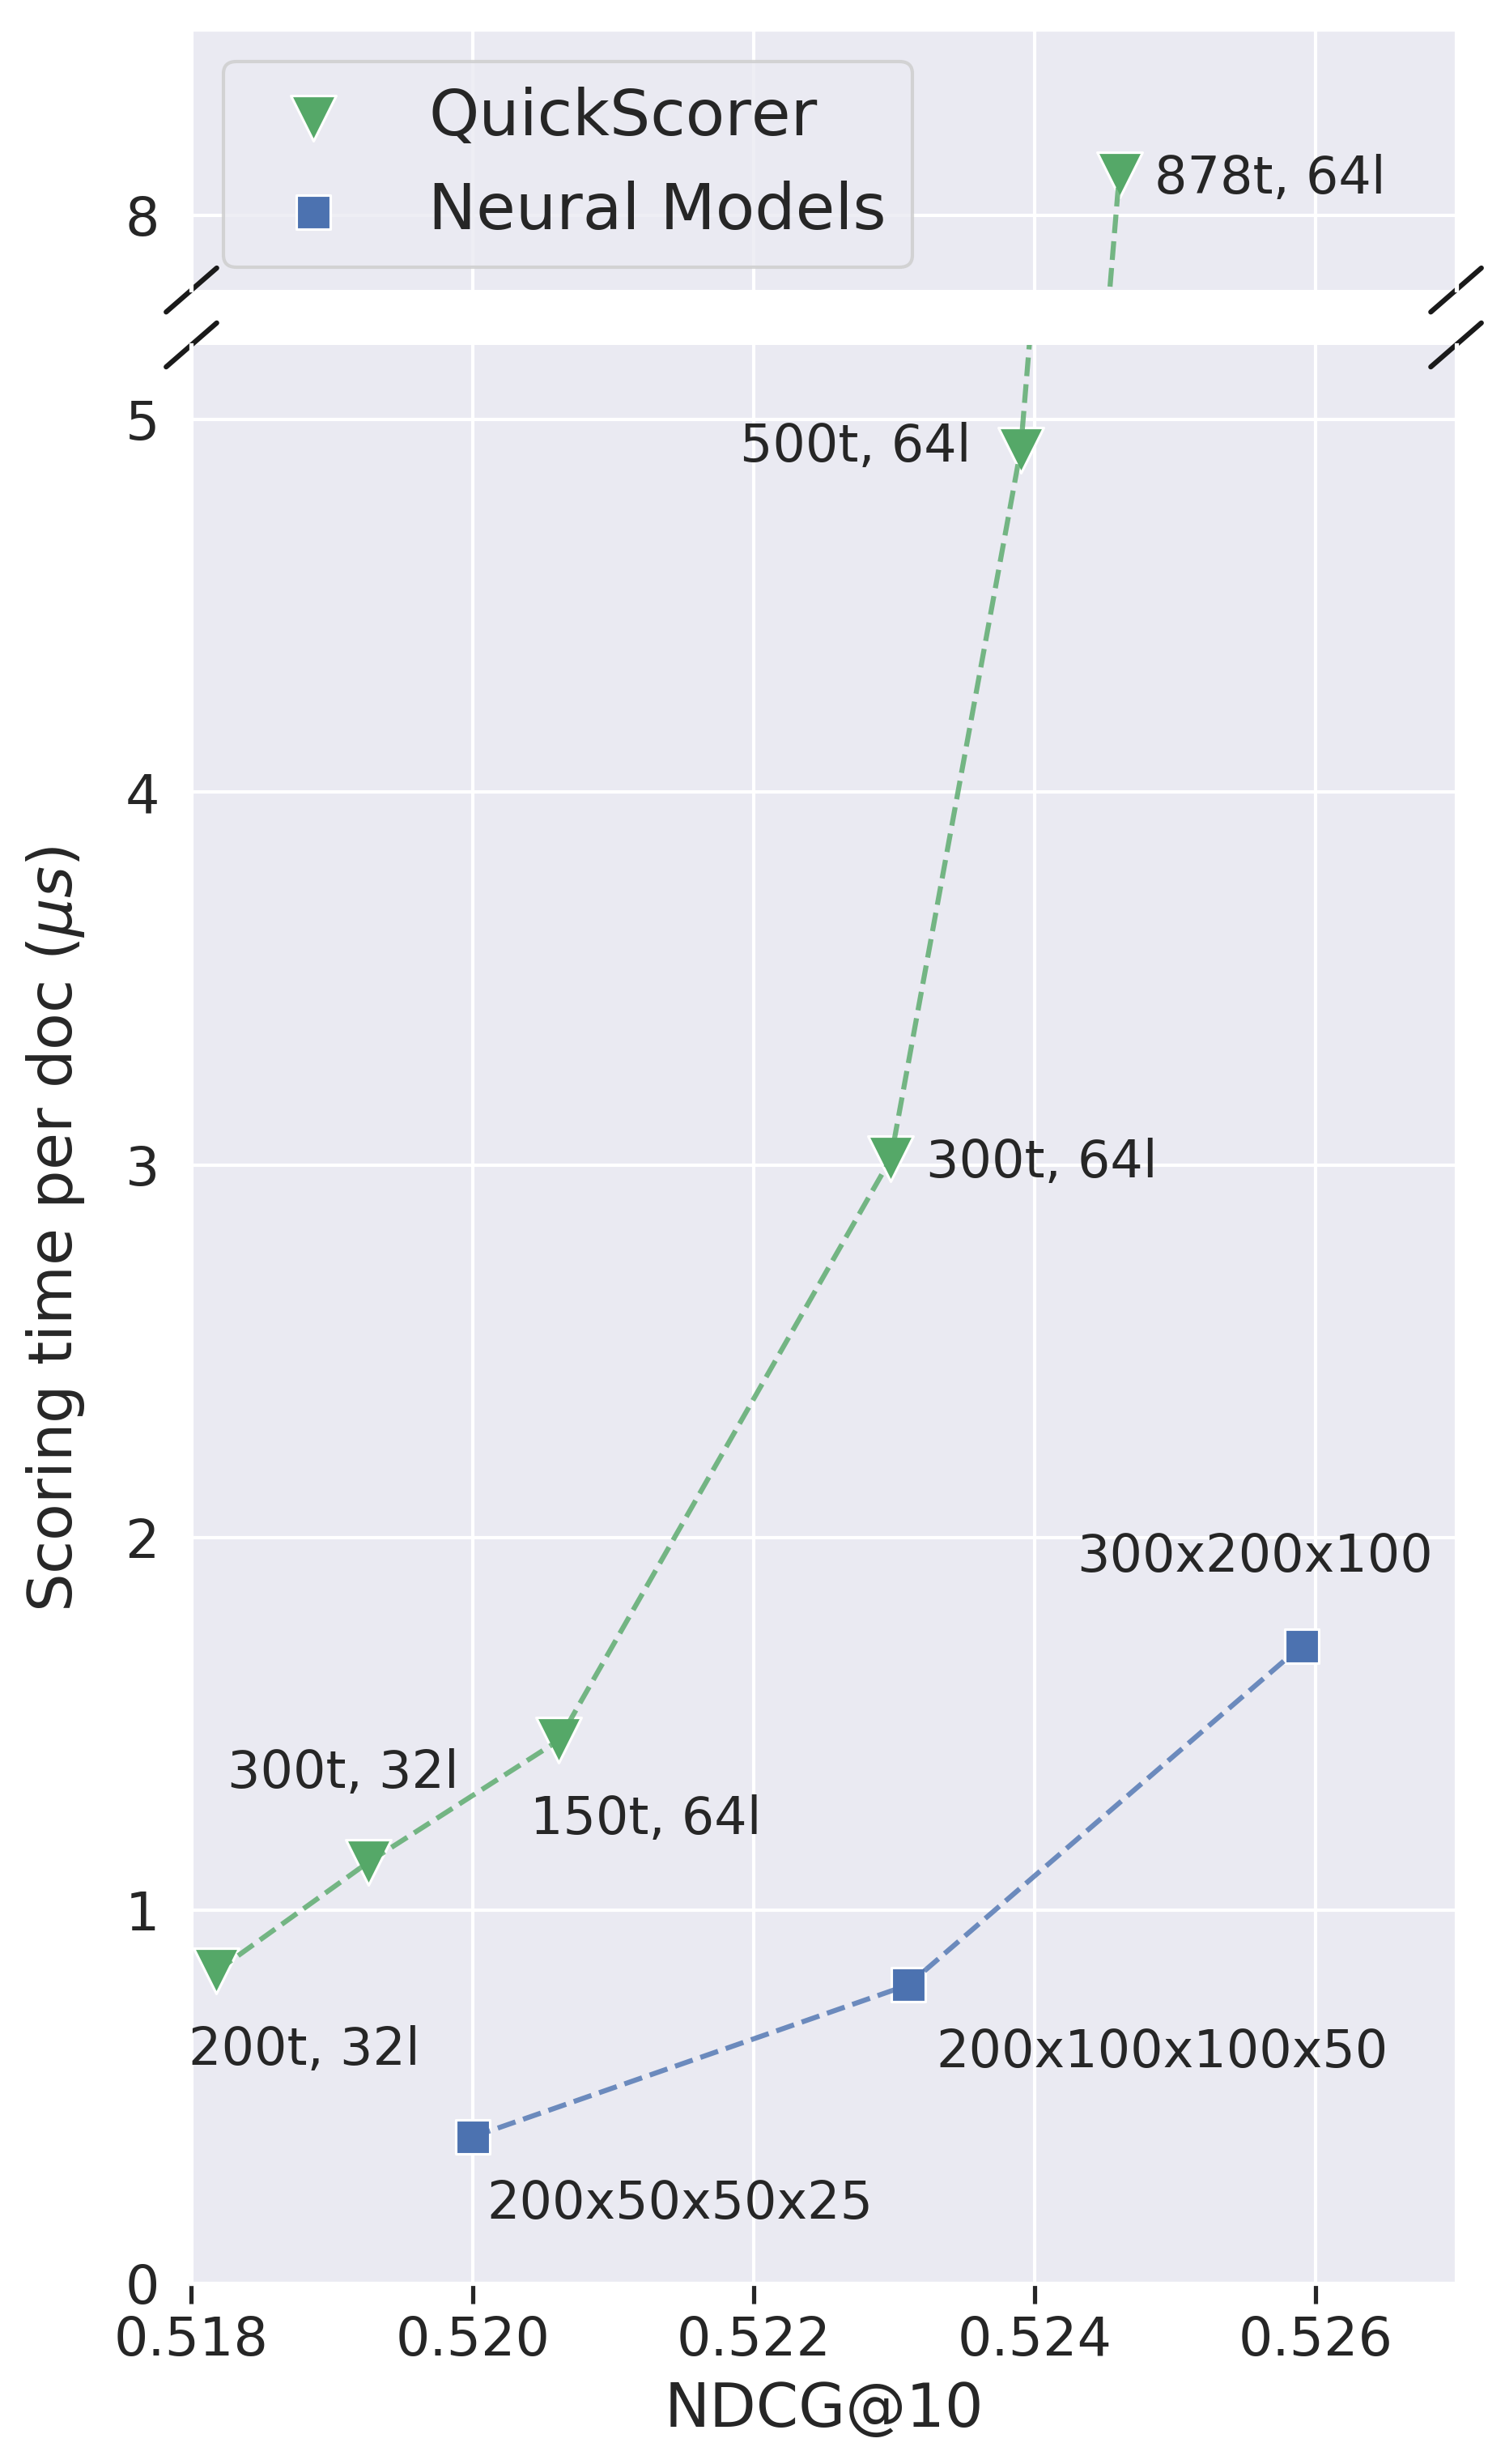
\includegraphics[width=\columnwidth]{imgs/msn30k_final_stretched_broken.png}
\caption*{\footnotesize{\msn}}
\end{minipage}%
\begin{minipage}[b]{0.517\columnwidth}
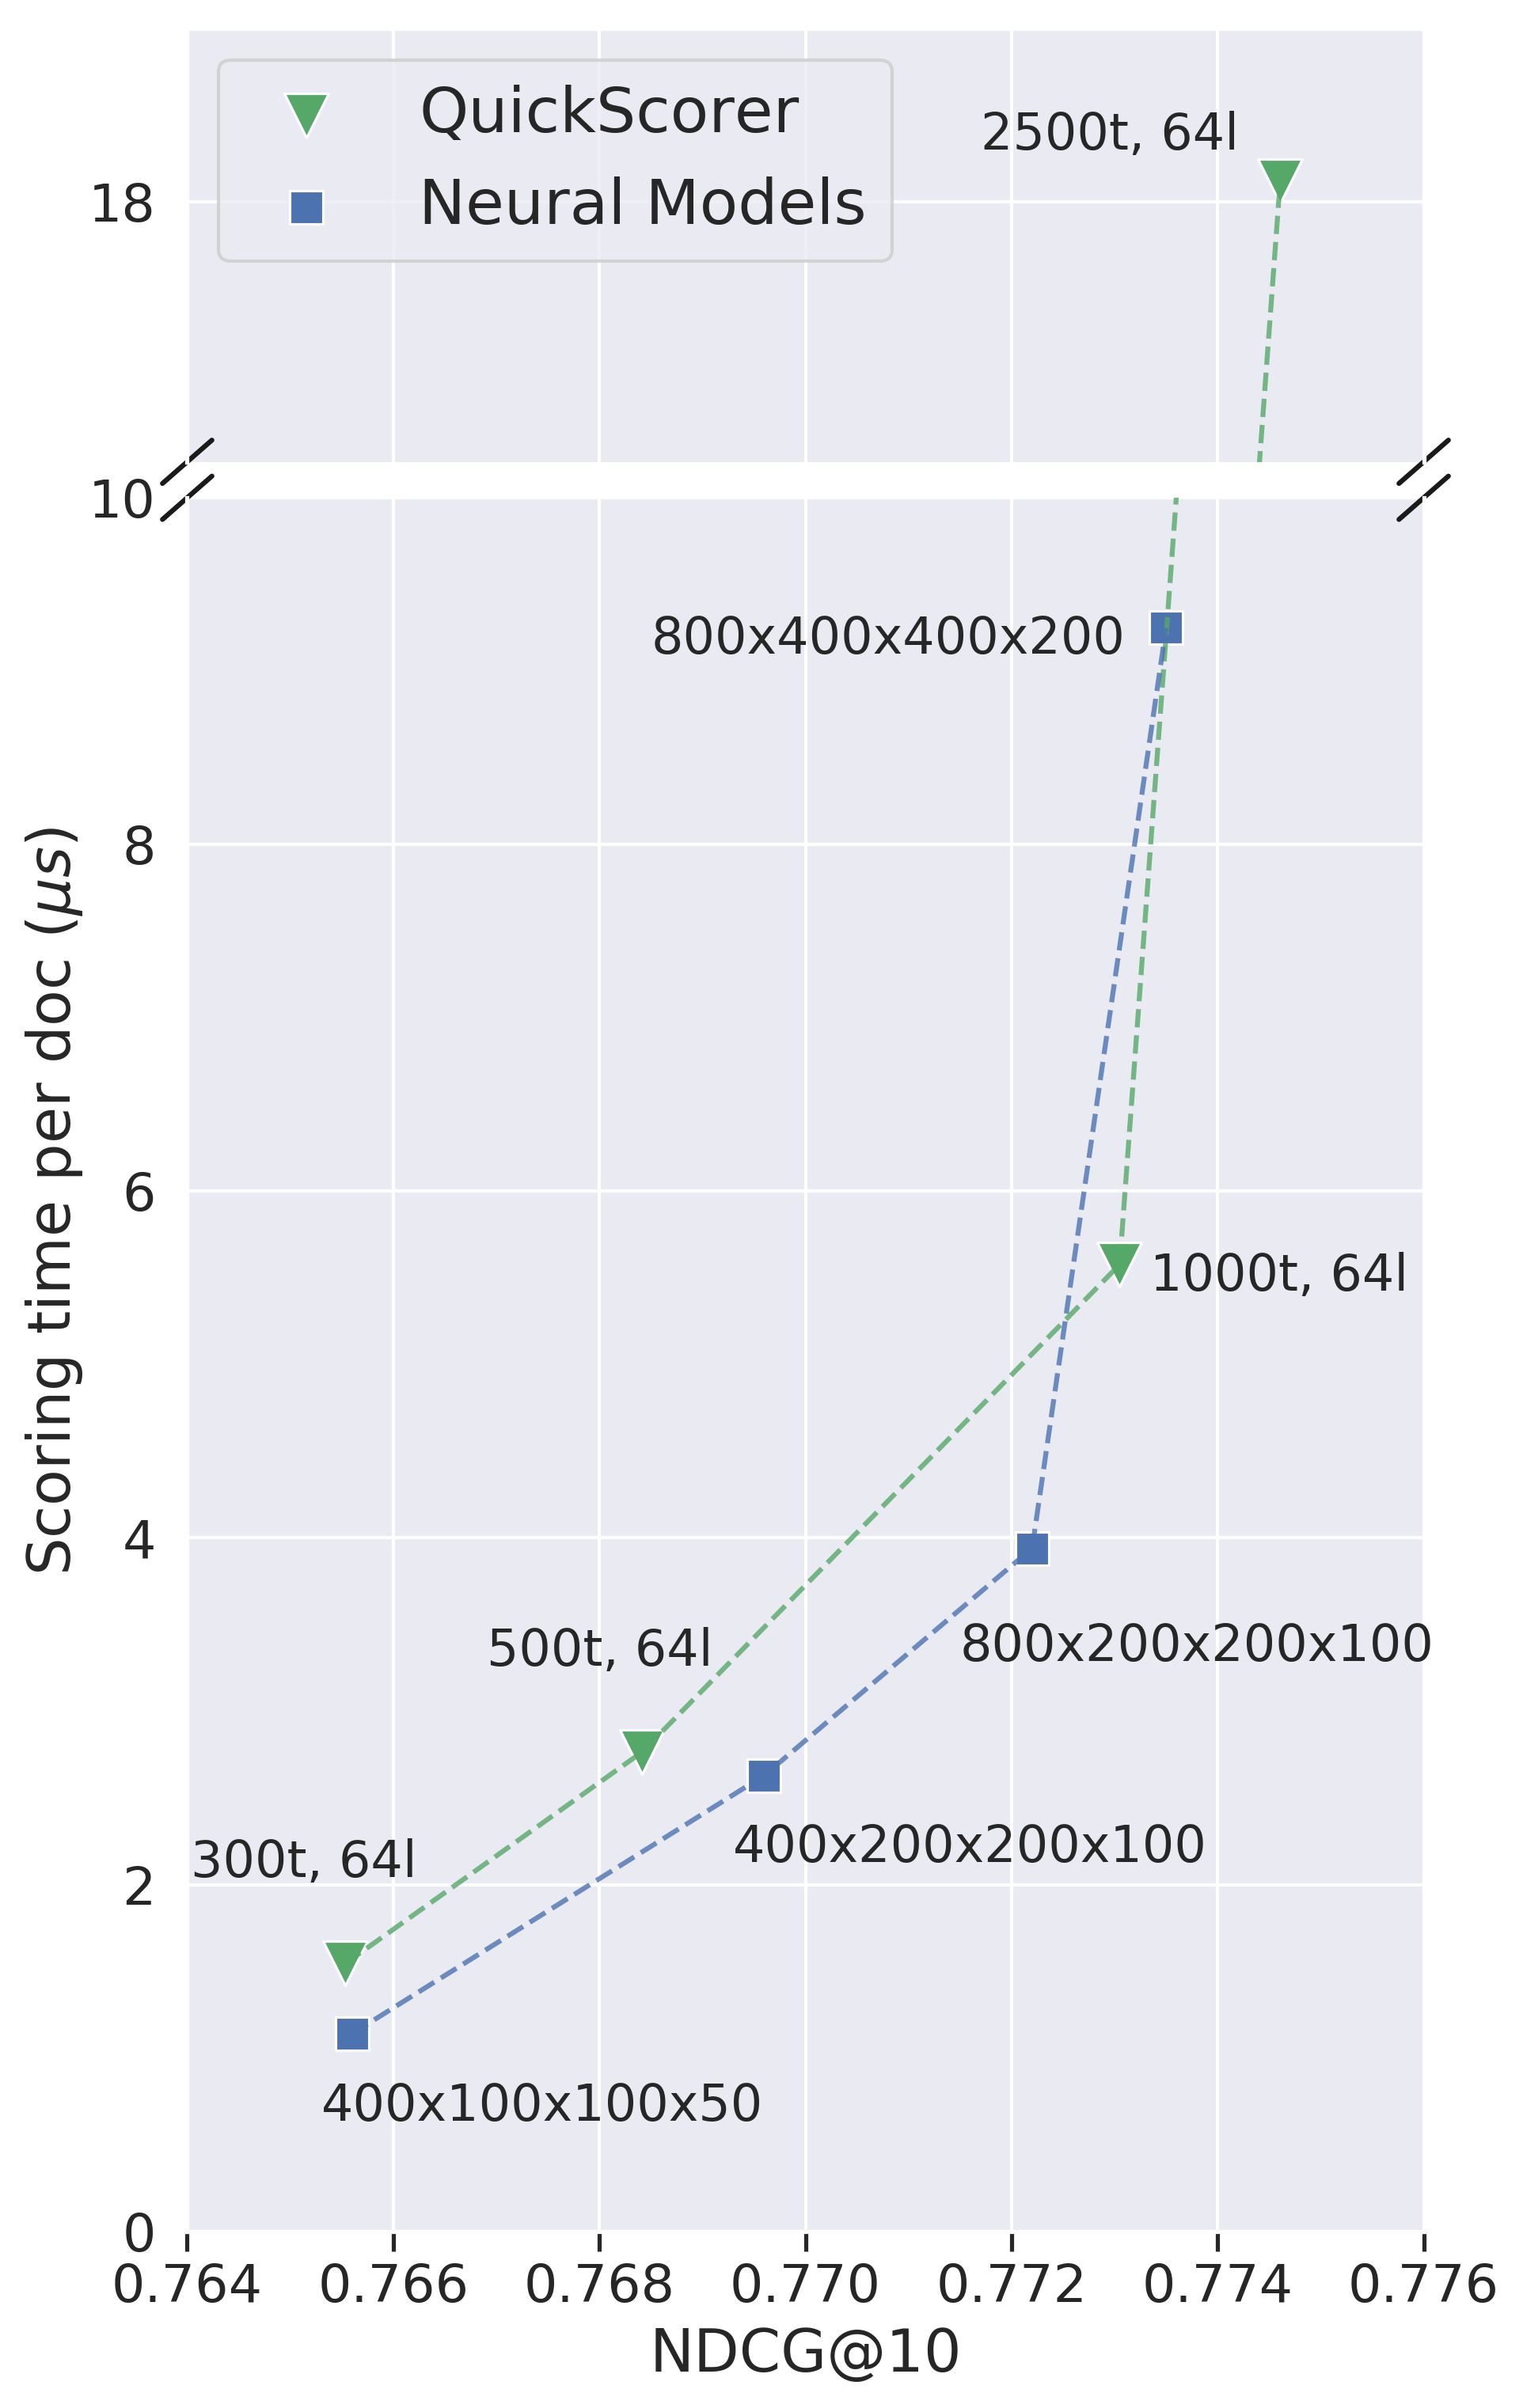
\includegraphics[width=\columnwidth]{imgs/istella_final_stretched_broken.png}
\caption*{\footnotesize{\istella}}
\end{minipage}%
\caption{Comparison between neural networks and ensemble of regression tree on the \textit{high-quality retrieval} scenario.\label{fig:hq}}
\end{figure}
%\smallskip
\noindent \textbf{High-Quality Retrieval}.
The first scenario of our comparison involves models delivering high-quality ranking. As previously detailed, we consider a model (both neural and tree-based) to be in the high-quality ranking region if its NDCG@10 is at least the 99\% of the top-quality tree model with 64 leaves.
By following the experimental methodology described above, we first construct the Pareto frontier for the ensemble of regression trees (green line in Figure\ref{fig:hq}).
We then move to the design of the neural network models. We can estimate the execution time of a neural model whose first layer is sparse with our time predictors. In particular, in Table~\ref{table:msn_final} we report the estimated execution time for the dense architecture, the relative impact of the first layer on the overall execution time, and the predicted execution time after pruning the first layer.
We always assume the sparsity of the first layer in the final model to be above $95\%$, so that its impact on the overall execution time is negligible. Our experiments show that this level of sparsity does not hamper the ranking capability of the model.
Observe that our time predictors permit to locate a neural model on the $y$-axis of the effectiveness-efficiency plot without any computational effort, analytically computing it given the architectures of network. 
Once we have designed our models to compete with the tree-based ones, we train and prune them, according to the methodology listed in Section~\ref{subsec:expsetup}.
\begin{table}[b]
	\centering
	\adjustbox{max width=\columnwidth}{
	\begin{tabular}{llrrrr}
		\toprule
		\multirow{2}{*}{Dataset} & \multirow{2}{*}{Model} & Sc. Time  & \nth{1} layer & Predicted Pruned   \\
		&& ($\mu s$/doc) & impact (\%)& Sc. Time  ($\mu s$/doc) \\
		\midrule	
		\multirow{3}{*}{\msn} & 300$\times$200$\times$100 & 2.4 & 30 &  1.7 \\
		&\footnotesize 200$\times$100$\times$100$\times$50 & 1.3 & 39 & 0.8 \\
		&200$\times$50$\times$50$\times$25 & 0.9 & 58 & 0.4\\
 		\midrule	
 		\multirow{3}{*}{\istella} & \footnotesize800$\times$400$\times$400$\times$200& 11.9 & 23 &  9.1 \\
		&\footnotesize800$\times$200$\times$200$\times$100	& 6.5 & 41 & 	3.8 \\
		&300$\times$200$\times$100 & 2.8 & 41 & 1.6	\\
		\bottomrule
	\end{tabular}}
	\caption{Prediction of model scoring time (Sc. Time) when pruning the first layer, in \emph{High Quality Retrieval}.  }
	\label{table:msn_final}
\end{table}

Figure~\ref{fig:hq} illustrates the comparison on a effectiveness-efficiency plot between neural models and ensemble of regression trees scored with QuickScorer. On the $x$-axis we report the NDCG@10 on the test set, and on the $y$-axis the scoring time per document in $\mu s$. First, we observe that the predicted times reported in Table~\ref{table:msn_final} coincide with real scoring time, confirming the precision of our theoretical approach. Hence, our methodology allows to train exclusively the required architectures. Secondly, neural models can outperform tree-based models in scoring documents, both in terms of effectiveness and efficiency. The neural Pareto-optimality, reported in blue in  Figure~\ref{fig:hq}, lays below the tree-based one (in green), either on the \msn dataset and on \istella. On the \msn dataset, for example, the 300$\times$200$\times$100 architecture is $4.4$x faster than the $878$-trees model and it also provides a higher retrieval quality. Furthermore, the 200$\times$50$\times$50$\times$25 architecture is the fastest model respecting the quality constraint on this dataset. The same consideration holds for \istella, where the fastest model respecting the imposed quality constraint is a neural network (400$\times$200$\times$200$\times$100).
On this dataset, neural models still outperform ensemble of regression trees on a large portion of the selected effectiveness-efficiency space, even if tree-based model deliver a slightly superior performance in the top performing region.
This leaves space for research work to further improve the quality of this approximation. 
%For the sake of fairness, we point out that struggling at high level of retrieval quality is a general drawback of neural models, but it is also the only one, as detailed discussed in Section~\ref{sec:conclusions}.	
%Considering the top performing models on the \msn da the most effective models: ERT $600, 64$, NDCG@10 $0.5291$,  and $300x200x100$ sparse at the $98.6$ in the first layer, NDCG@10 $0.5258$. The gap between the two models in terms of NDCG@10 suggests than when aiming to maximize the retrieval quality, tree-based models are still to prefer to NNs, even if the price can be a $10x$ larger execution time w.r.t. to neural models.

% Observe that the models respect the predicted execution time reported in Table~\ref{table:\msn_final}, confirming the validity of our theoretical approach. Observe also  that neural models outperform the ensemble of regression trees scored with QuickScorer on \msn at any point of the efficiency-effectiveness trade-off; this can be evicted by fact that the neural Pareto curve always stands below the tree Pareto curve. The difference is especially evident between the two top NDCG@10 models. The 300x200x100 architecture is $4.4x$ faster than the 878-trees model, and $0.002$ more accurate in terms of NDCG@10, which is a relevant gap in terms of retrieval quality. For the sake of fairness, we point out the only possible disadvantage of using neural models; let us consider the most effective models: ERT $600, 64$, NDCG@10 $0.5291$,  and $300x200x100$ sparse at the $98.6$ in the first layer, NDCG@10 $0.5258$. The gap between the two models in terms of NDCG@10 suggests than when aiming to maximize the retrieval quality, tree-based models are still to prefer to NNs, even if the price can be a $10x$ larger execution time w.r.t. to neural models. 
% Then, we train an prune them; the most successful training configuration we found is to train for $250$ epochs,  using the dropout with  $p=0.1$ just on the first layer, no weight decay, and scheduling to multiply the learning rate with $\gamma = 0.5$ at epochs $\{90, 130, 180 \}$. The pruning phase consist of a total of $250$ epochs:  $60$ of pruning-retraining, with $10$ epochs of fine-tuning between one pruning iteration and the successive, and $190$ of solely fine-tuning. The training hyper-parameters remain the same as in the previous training phase. 
% In Figure~\ref{fig:\istella_high_quality} we report the comparison between the neural and tree-based Pareto Optimality curve. Even on a complex dataset as \istella, the neural models results more convenient on a large portion of the curve. In particular, NNs always to be preferred when the NDCG@10 is below $0.7220$. The tree-based models instead results advantageous with top-quality effectiveness requirements, \textit{i.e.}, NDCG@10 $ > 0.7740$, which NNs struggles to obtain. Observe also that the top performing ensemble of regression trees, ERT $2500, 256$, NDCG@10 0.7821, largely outscores our top performing model, the $800x400x400x200$, NCGG@10 0.7734 . 





\smallskip
\noindent \textbf{Low-Latency Retrieval}. We now compare neural models and ensemble of regression trees on a low-latency retrieval setting, \textit{i.e.}, a scenario requiring the scoring time to be lower than $0.5 \mu s$ per document. The Pareto Optimality curve for the ensemble of regression trees is drawn in green in Figure~\ref{fig:lowlat}. We use this plot to identify the latency constraints for our neural networks. Our proposed methodology permits to precisely estimate the execution time of a model, before carrying out the costly training-pruning phase. In Table~\ref{table:msn_lowq}, we demonstrate the usage of our methodology. As we did for the \emph{high-quality retrieval} use case (Table~\ref{table:msn_final}), we report the predicted execution time for the dense architecture, the relative impact of the first layer and the predicted time after sparsification. We still consider the impact of the first layer to be negligible.
%The models involved in this latency-bound use case are smaller, in order to match the latency constraints. Anyway, we experimentally verify that the pruning technique is capable to sparsify the first layer up to 95\%, annihilating the contribute of the first layer to the overall execution time. }
\begin{table}[b]
	\centering
	\adjustbox{max width=\columnwidth}{
	\begin{tabular}{llrrrr}
	%\resizebox{\columnwidth}{!}{
		\toprule
		%\multirow{2}{*}{Model} &    \multicolumn{2}{c}{Scoring Time ($\mu s$/doc)} \\
		%\cmidrule{2-3}
		\multirow{2}{*}{Dataset} & \multirow{2}{*}{Model} & Sc. Time  & \nth{1} layer   & Predicted Pruned  \\
		&& ($\mu s$/doc) & impact (\%)& Sc. Time  ($\mu s$/doc) \\
			\midrule
		%100x75x75x10 & 0.7 & 0.43 & 0.4\\
		\multirow{3}{*}{\msn}&100$\times$50$\times$50$\times$25 & 0.6 & 56 & 0.3\\
		&100$\times$25$\times$25$\times$10 & 0.5 & 71 & 0.2\\
		&50$\times$25$\times$25$\times$10 & 0.3 & 65 & 0.1 \\
 		\midrule
		\multirow{3}{*}{\istella}&  200$\times$75$\times$75$\times$25&1.6 & 61 &  0.6 \\
		&100$\times$75$\times$75$\times$10& 0.9 & 55 & 	0.4 \\
 		&100$\times$50$\times$50$\times$10 & 0.8 & 67 & 0.3	\\
		\bottomrule
	\end{tabular}
	}
	\caption{Prediction of model scoring time (Sc. Time) when pruning the first layer, in \emph{Low-Latency Retrieval}.\label{table:msn_lowq}}
\end{table}


\begin{figure}[t]
\begin{minipage}[b]{0.5\columnwidth}
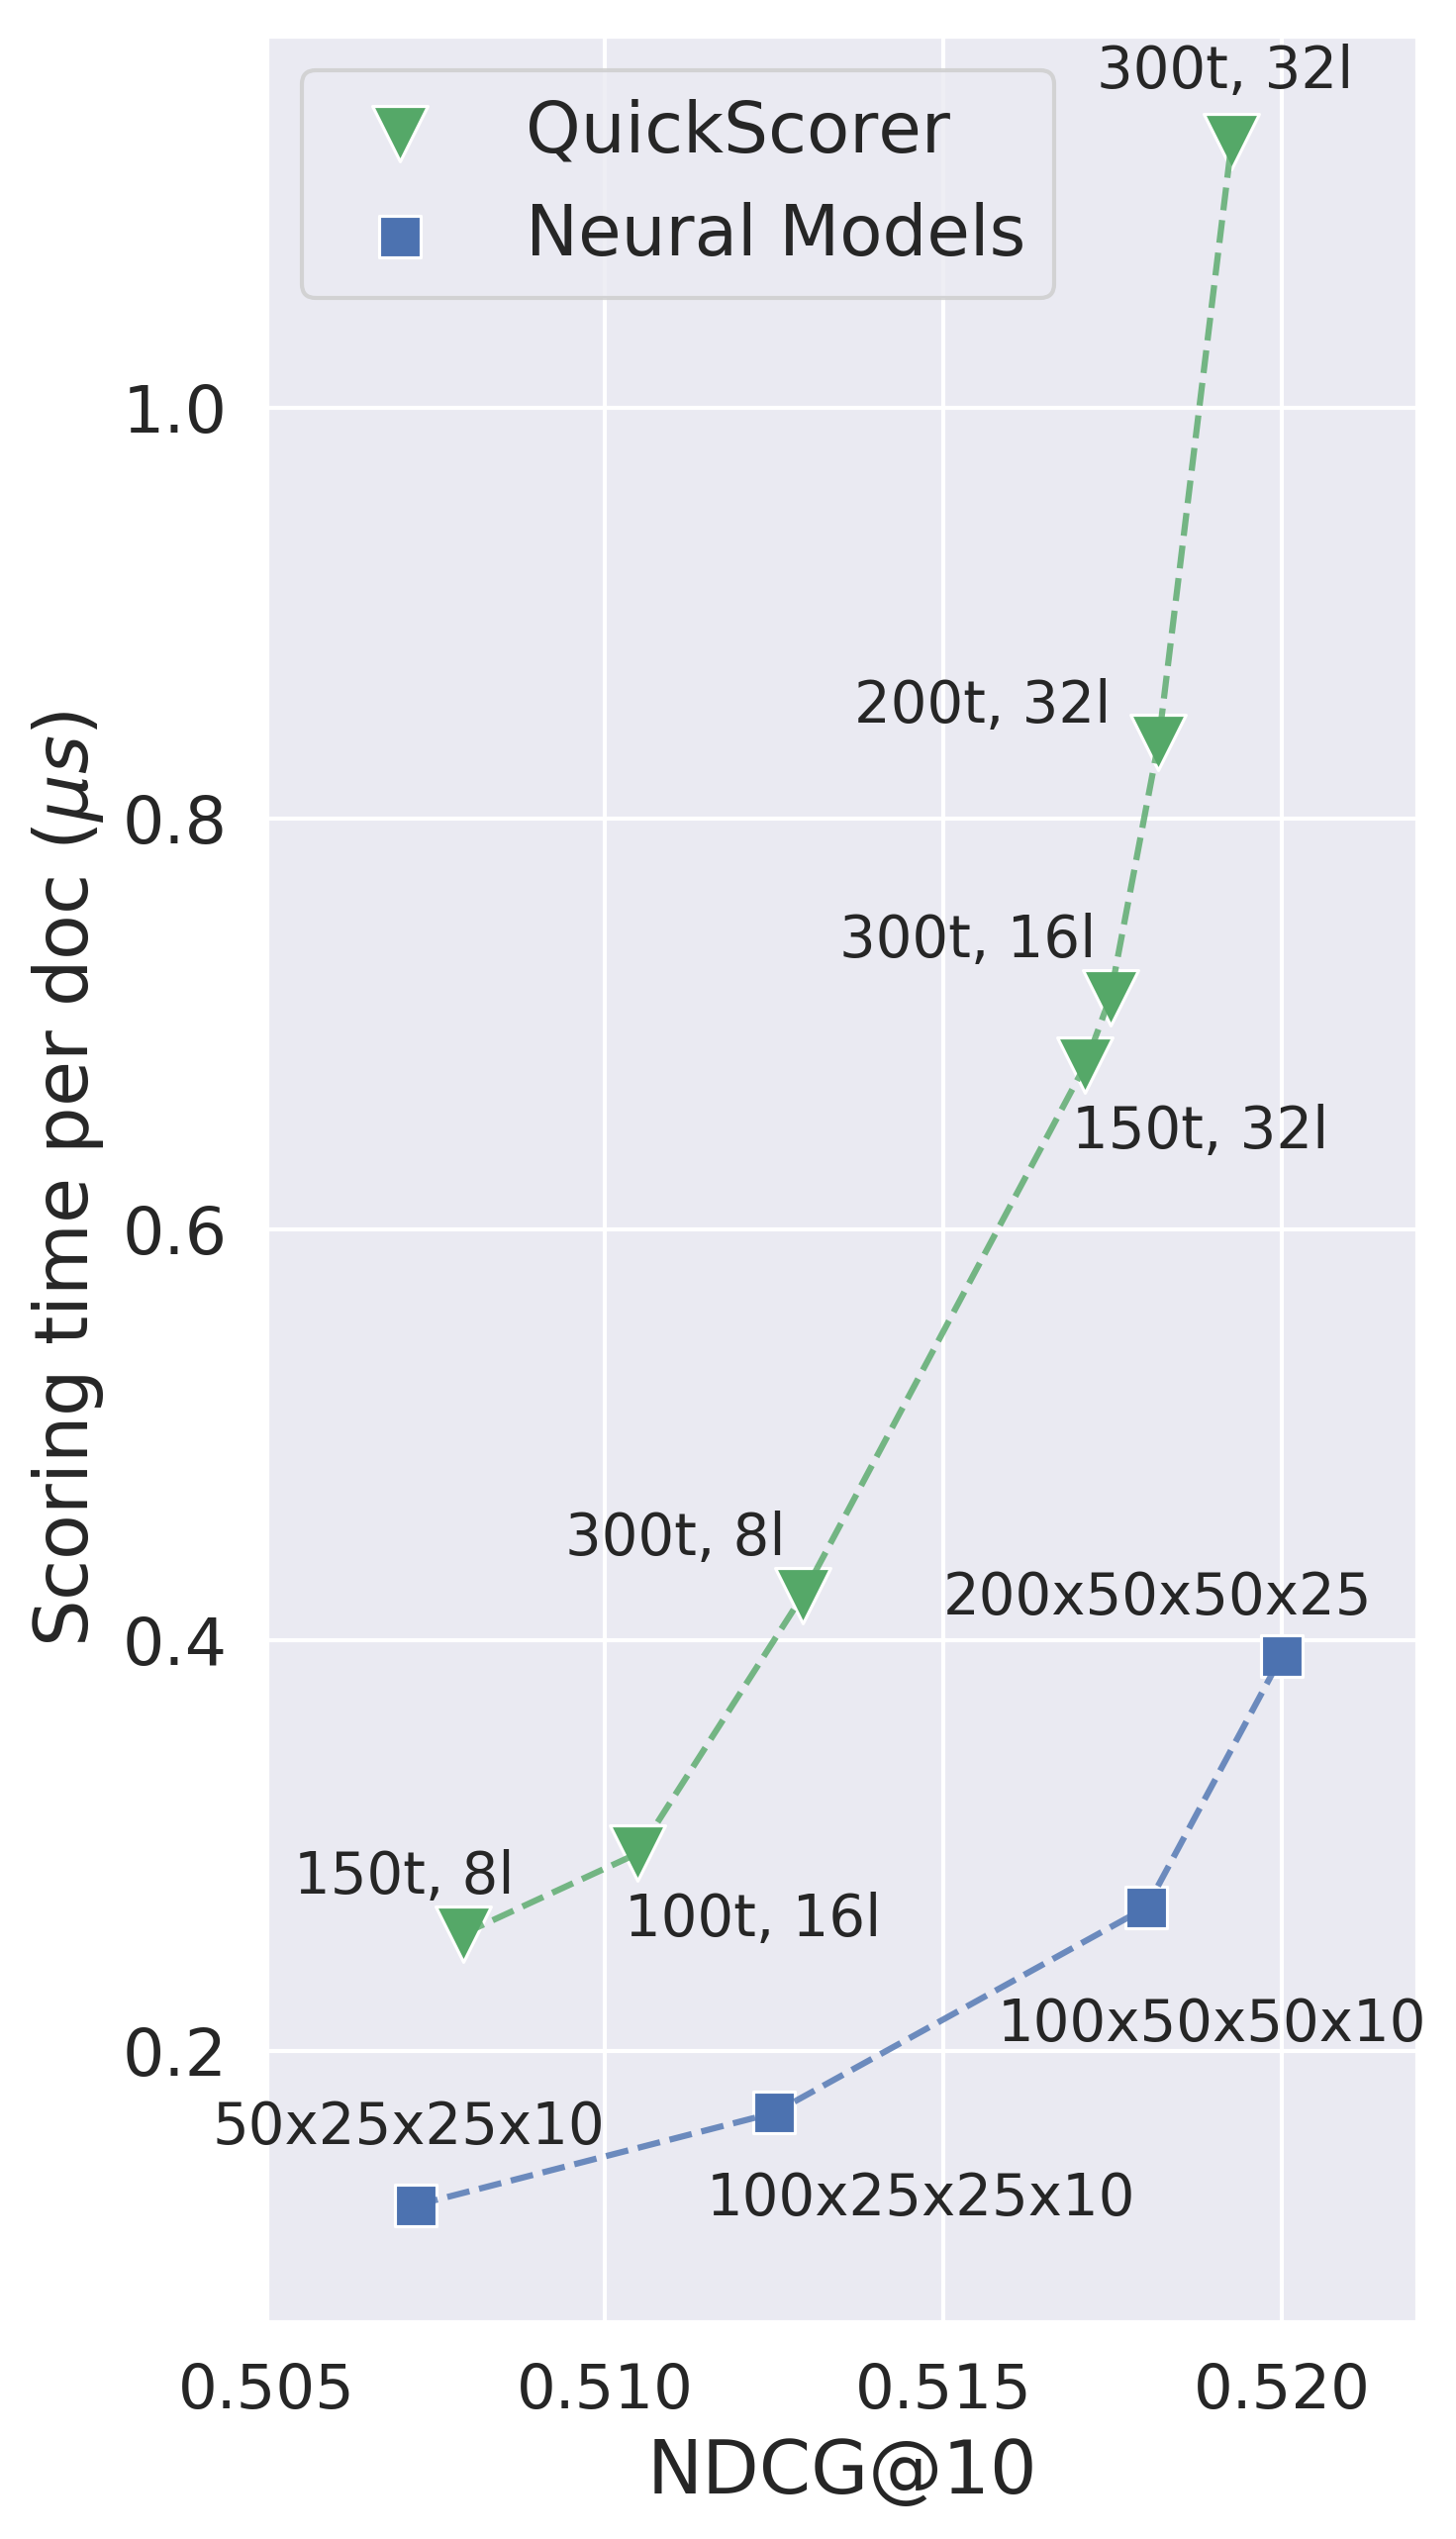
\includegraphics[width=\columnwidth]{imgs/low_effectiveness_msn30k_stretched.png}
\centering 
\caption*{\footnotesize{\msn}}
\end{minipage}%
\begin{minipage}[b]{0.51\columnwidth}
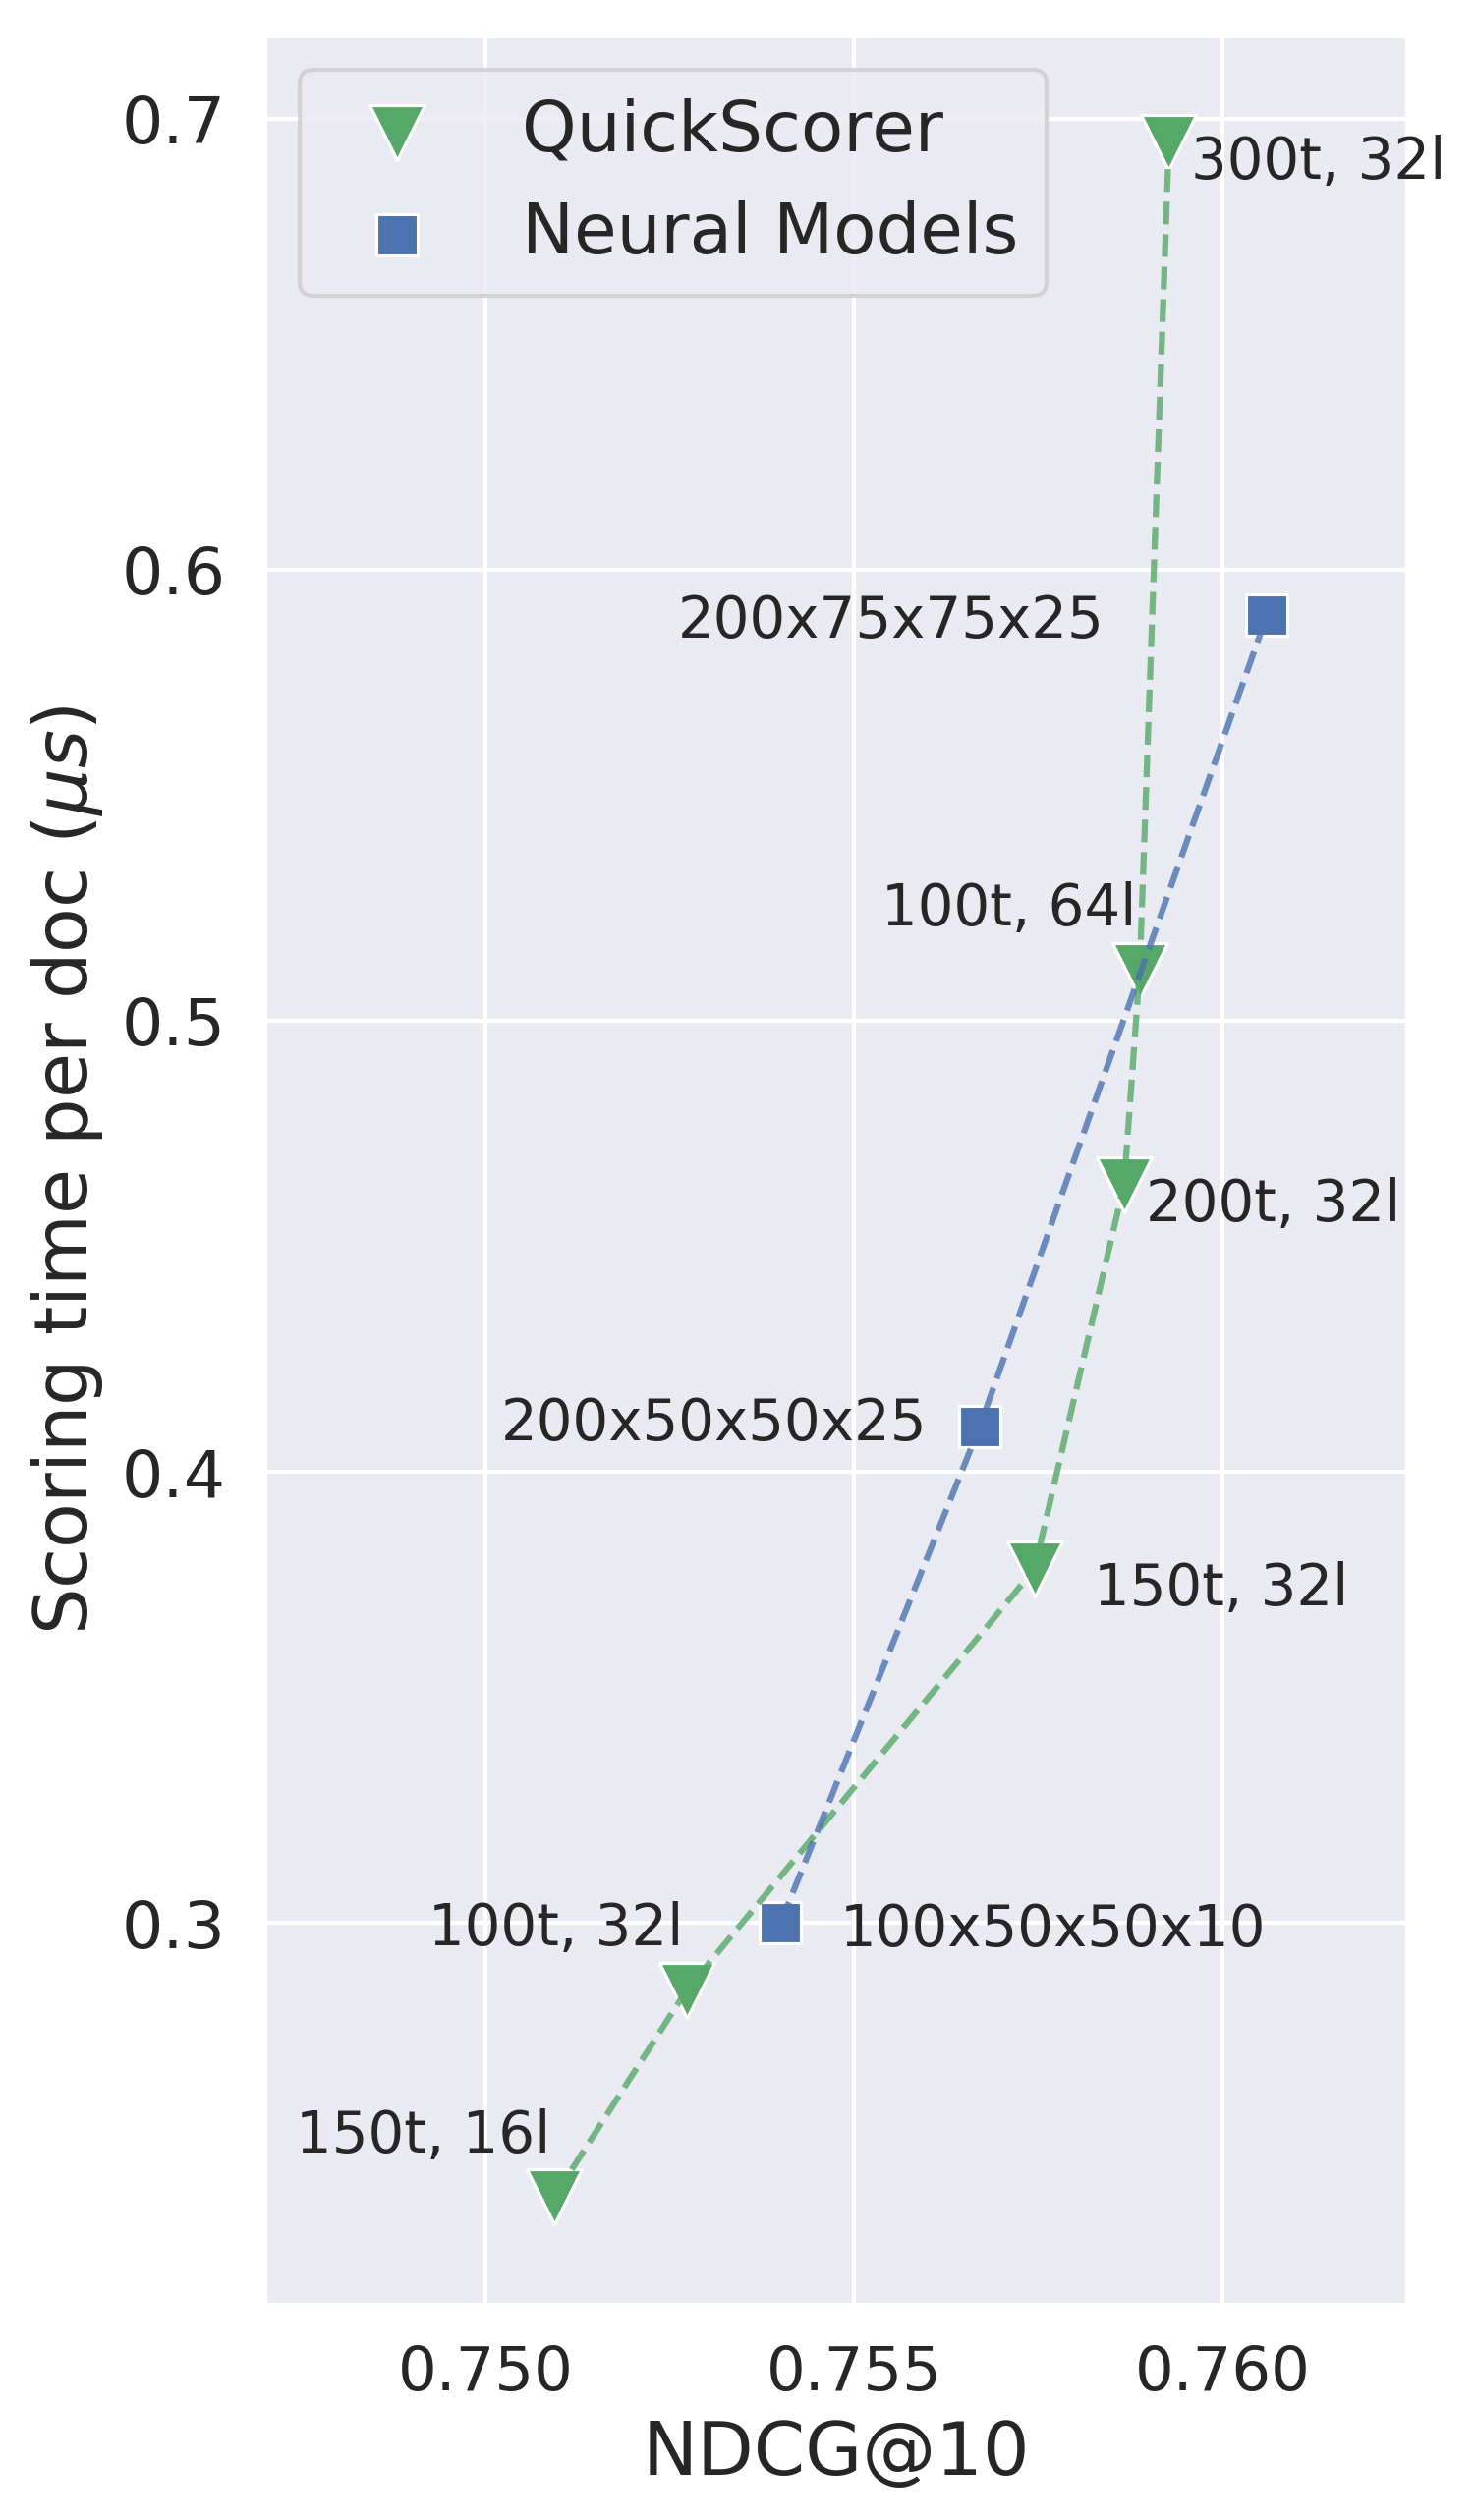
\includegraphics[width=\columnwidth]{imgs/low_effectiveness_istella_stretched.png}
\centering 
\caption*{\footnotesize{\istella}}
%\subcaption{Another subfigure}
\end{minipage}%
\caption{Comparison between neural networks and ensemble of regression tree on the \textit{low-latency retrieval} scenario.}
\label{fig:lowlat}
\end{figure}



Figure~\ref{fig:lowlat} illustrates the comparison between neural model and ensemble of regression trees when dealing with low-latency constraints. Even in this case, our methodology permits to create neural networks that  outperform ensembles of regression trees. On the \msn dataset, neural models dominate over tree-based models, as happened for the \textit{high-quality} use case. In fact,  the Pareto frontier of neural models (in blue) always lies below the tree-based one, confirming the superiority of our technique on this dataset (left side of Figure~\ref{fig:lowlat}). In particular, the 200$\times$50$\times$50$\times$25 architecture is $3$x faster than the regression forest with $300$ trees and $32$ leaves, while being also more precise in terms of NDCG@10. On the \istella dataset (right side of Figure~\ref{fig:lowlat}, the performance of our neural models can be considered on pair with tree-based models. In fact, the two Pareto frontiers intersect in this portion of the efficiency-effectiveness trade-off. Despite that, neural networks  still provide the most effective model respecting the time requirement (200$\times$75$\times$75$\times$25). 
This dataset confirms to be troublesome for neural models, as witnessed in the high-quality retrieval scenario. 
% We leave for future work the investigation of distillation techniques tackling these difficulties on this specific dataset.
%\fnote{la chiusura con un future work la eviterei. FM}

% Once again, we design our neural model just using our time predictors. 
% We keep the $200x50x50x25$ neural model from the previous experimental setting and devise three more architectures. 

% %mainly composed by trees with $8$ or  $16$ leaves. A minor number of leaves and/or trees, in fact, allows for faster scoring with QuickScorer, at the price of a reduced expressiveness. For what concerns the neural models, observe that 
% %the $200x50x50x25$ model previously developed already matches the requirement of  $ 0.5 \mu s$ of scoring time per document. Furthermore, we develop three more models using the same methodology as before: we estimate the execution time of the pruned models as the total execution time subtracted with the contribution of the first layer. We highlight that the models' design is completely experiments-free, thus costless. 

% In Table~\ref{table:\msn_lowq} we report the predicted execution times after the sparsification; because of the reduced sizes of the layers, we assume our processor to perform at 60 GFLOP/s, as also suggested by Figure~\ref{fig:heatmap}. We train an then prune the resulting models; the training and pruning recipes are exactly the same as in the \textit{High Quality Retrieval} use case. The only difference is that  we use medium or low aggressive pruning ($s \in [ 0.5, 1.0]$) since these architectures have few parameters and aggressively sparsify them could cause unbearable performance degradation. In Figure~\ref{fig:\msn_lowlat} we report both the Pareto Optimality curves. As for the high quality retrieval, the real scoring times reflect the predicted scoring time reported in Table~\ref{fig:\msn_lowlat}. %The very-low effort time analysis allows to train only a reduced number of models, tearing down the resource needed for training, \textit{i.e.}, time, money, energy. 
% Even in this case, the neural Pareto Optimality curve always appears below the tree Pareto Optimality. As an example, the architecture $200x100x100x50$ is $0.002$ more accurate than the $300t, 32l$ tree-based model, while being $3x$ times faster. The validity of our theoretical-based approach to efficiency is confirmed even in this use case, especially considering that the model design phase involves no computational effort, tearing down the resource needed for training, \textit{i.e.}, time, money, energy. 
 %As for \msn, we now move to compare tree-based and neural model whose scoring time is about $ 0.5 \mu s$ per document. The profile of the Pareto Optimality curve for ensemble of regression trees is reported in green in Figure~\ref{fig:lowlat\istella}. Following the same procedure we follow during the all experimental evaluation, we use our time predictor to devise the models that we will train, as reported in Table~\ref{table:\istella_lowlat}. To train and prune the architecture we use the same parameters configuration as in \textit{High Quality Retrieval}; the pruning aggressiveness is reduced because of the small size of the models. We report our results in Figure~\ref{fig:lowlat\istella}: as shown, neural models are capable to compete with tree-based ones even with low-latency requirements on the \istella dataset. 






% \subsection{MSN 30K }
% In this section we report the results of our experiments on the \msn dataset~\cite{DBLP:journals/corr/QinL13}, a well-established benchmark to monitor the evolution of LtR techniques. The dataset is composed  by more than 30,000 queries, with about 120 documents per query; each document is a vector of 136 features. The whole dataset is split into train-validation-test according to a 60\%-20\%-20\% criterion. 

% As already reported in Table~\ref{table:64vs256leaves}, the most effective ensemble of regression trees  we could obtain on \msn is a model with 600-trees and 256 leaves per tree, reaching 0.5291 of NDCG@10. We used this model as \textit{teacher} for all of our neural models. 

% \smallskip
% \noindent \textbf{High Quality Retrieval}
% We begin our comparison between tree-based and neural models on \msn from models whose NDCG@10 is the in the 1\% of the top quality tree model with 64 leaves. 
% Following the guidelines in the preamble at the beginning of this section, we first construct the Pareto Optimality curve for the ensemble of regression trees, reported in green in Figure\ref{fig:\msn_highperf}. Hence, we move to the design of our hybrid sparse-dense neural models; as anticipated in the preamble, we can estimate the execution time of a first layers sparse neural model with our time predictors, as reported in Table~\ref{table:\msn_final}. We always assume the sparsity of the first layer in the final model to be above $95\%$, so that its impact on the overall execution time is negligible. 
% Observe that this method allows us to locate a neural  model on the y-axis of the effectiveness-efficiency plot without any computational effort, just using the architecture of the network.

% Once we have designed our models to compete with the tree-based ones, we train and prune them. In the training phase, additionally to the information specified in the preamble, we highlight that we did not use dropout nor weight decay on our models: we train for $100$ epochs, and  multiply the learning rate by $\gamma = 0.1$ at epochs $\{50, 80\}$. We employ an aggressive pruning ($s=1.5$) for all the models except for the smallest one, for which we use $s=1.0$. The overall pruning procedure lasts $100$ epochs; we prune once and retrain for $10$ epochs for the first $80$ epochs, then we solely fine-tune for the last $20$. During the fine-tuning epochs, the hyper-parameters, learning rate, weight decay, etc..,  are set as in the training phase. In Figure ~\ref{fig:\msn_highperf} we draw the Neural Pareto Optimality curve. Observe that the models respect the predicted execution time reported in Table~\ref{table:\msn_final}, confirming the validity of our theoretical approach. Observe also  that neural models outperform the ensemble of regression trees scored with QuickScorer on \msn at any point of the efficiency-effectiveness trade-off; this can be evicted by fact that the neural Pareto curve always stands below the tree Pareto curve. The difference is especially evident between the two top NDCG@10 models. The 300x200x100 architecture is $4.4x$ faster than the 878-trees model, and $0.002$ more accurate in terms of NDCG@10, which is a relevant gap in terms of retrieval quality. For the sake of fairness, we point out the only possible disadvantage of using neural models; let us consider the most effective models: ERT $600, 64$, NDCG@10 $0.5291$,  and $300x200x100$ sparse at the $98.6$ in the first layer, NDCG@10 $0.5258$. The gap between the two models in terms of NDCG@10 suggests than when aiming to maximize the retrieval quality, tree-based models are still to prefer to NNs, even if the price can be a $10x$ larger execution time w.r.t. to neural models. 

% \begin{table}[]
% 	\centering

% 	\adjustbox{max width=\columnwidth}{
% 	\begin{tabular}{lrrrr}
% 	%\resizebox{\columnwidth}{!}{
% 		\toprule
% 		%\multirow{2}{*}{Model} &    \multicolumn{2}{c}{Scoring Time ($\mu s$/doc)} \\
% 		%\cmidrule{2-3}
% 		\multirow{2}{*}{Model} & Scoring Time  & \nth{1} layer   & Predicted Pruned  \\
% 		& ($\mu s$/doc) & impact (\%)& Scoring Time  ($\mu s$/doc) \\
% 		\midrule
% 		\sc{800x400x400x200}& 11.9 & 0.23 &  9.1 \\
% 		800x200x200x100	& 6.5 & 0.41 & 	3.8 \\
% 		300x200x100 & 2.8 & 0.41 & 1.6	\\
%  		\bottomrule
% 	\end{tabular}
% 	  }
% 	\caption{Predicting the scoring time of Neural Models for High Quality Retrieval on \istella, assuming the first layer to be sparse.  }
% 	\label{table:\istella_final}

% \end{table}


% \begin{figure}
% 	\centering
% 	\includegraphics[width=\columnwidth]{imgs/\msn_final.png}
% 	\caption{High Quality Retrieval comparison between Additive Ensemble of Regression Trees, scored with QuickScorer, and Neural Models on \msn }
% 	\label{fig:\msn_highperf}
% \end{figure}


% \smallskip
% \noindent \textbf{Low Latency Retrieval}
% We now move to the compare neural models and ensemble of regression trees on low latency constraints, \textit{i.e.}, scoring time below $0.5 \mu s$ per document. 	
% The Pareto Optimality curve for the ensemble of regression trees is draw in green in Figure~\ref{fig:\msn_lowlat}. 
% Once again, we design our neural model just using our time predictors. 
% We keep the $200x50x50x25$ neural model from the previous experimental setting and devise three more architectures. 

% %mainly composed by trees with $8$ or  $16$ leaves. A minor number of leaves and/or trees, in fact, allows for faster scoring with QuickScorer, at the price of a reduced expressiveness. For what concerns the neural models, observe that 
% %the $200x50x50x25$ model previously developed already matches the requirement of  $ 0.5 \mu s$ of scoring time per document. Furthermore, we develop three more models using the same methodology as before: we estimate the execution time of the pruned models as the total execution time subtracted with the contribution of the first layer. We highlight that the models' design is completely experiments-free, thus costless. 

% In Table~\ref{table:\msn_lowq} we report the predicted execution times after the sparsification; because of the reduced sizes of the layers, we assume our processor to perform at 60 GFLOP/s, as also suggested by Figure~\ref{fig:heatmap}. We train an then prune the resulting models; the training and pruning recipes are exactly the same as in the \textit{High Quality Retrieval} use case. The only difference is that  we use medium or low aggressive pruning ($s \in [ 0.5, 1.0]$) since these architectures have few parameters and aggressively sparsify them could cause unbearable performance degradation. In Figure~\ref{fig:\msn_lowlat} we report both the Pareto Optimality curves. As for the high quality retrieval, the real scoring times reflect the predicted scoring time reported in Table~\ref{fig:\msn_lowlat}. %The very-low effort time analysis allows to train only a reduced number of models, tearing down the resource needed for training, \textit{i.e.}, time, money, energy. 
% Even in this case, the neural Pareto Optimality curve always appears below the tree Pareto Optimality. As an example, the architecture $200x100x100x50$ is $0.002$ more accurate than the $300t, 32l$ tree-based model, while being $3x$ times faster. The validity of our theoretical-based approach to efficiency is confirmed even in this use case, especially considering that the model design phase involves no computational effort, tearing down the resource needed for training, \textit{i.e.}, time, money, energy. 
 

% \begin{table}[]
% 	\centering

% 	\adjustbox{max width=\columnwidth}{
% 	\begin{tabular}{lrrrr}
% 	%\resizebox{\columnwidth}{!}{
% 		\toprule
% 		%\multirow{2}{*}{Model} &    \multicolumn{2}{c}{Scoring Time ($\mu s$/doc)} \\
% 		%\cmidrule{2-3}
% 		\multirow{2}{*}{Model} & Scoring Time  & \nth{1} layer   & Predicted Pruned  \\
% 		& ($\mu s$/doc) & impact (\%)& Scoring Time  ($\mu s$/doc) \\
% 			\midrule
% 		%100x75x75x10 & 0.7 & 0.43 & 0.4\\
% 		100x50x50x25 & 0.6 & 0.56 & 0.3\\
% 		100x25x25x10 & 0.5 & 0.71 & 0.2\\
% 		50x25x25x10 & 0.3 & 0.65 & 0.1 \\
%  		\bottomrule
% 	\end{tabular}
% 	  }
% 	\caption{Predicting the scoring time of Neural Models for Low Latency Retrieval on \msn, assuming the first layer to be sparse.  }
% 	\label{table:\msn_lowq}

% \end{table}


% \begin{figure}
% 	\centering
% 	\includegraphics[width=\columnwidth]{imgs/low_effectiveness_\msn.png}
% 	\caption{Low Latency Retrieval comparison between Additive Ensemble of Regression Trees, scored with QuickScorer, and Neural Models on \msn }
% 	\label{fig:\msn_lowlat}
% \end{figure}


% \subsection{\istella dataset}
% The second part of our experimental evaluation is performed on the \istella~\cite{lucchese2016post} dataset by Tiscali. In order to ease reproducibility, we pick the the \textit{small} version (\istella); it consists of a collection of 33,018 queries with an average of $103$ documents per query. Each document-query pair is represented by $220$ features. The train-validation-test split	respects the same pattern as \msn, \textit{i.e.}, 60\%-20\%- 20\%. 

% As first step, we perform a grid search on the hyper-parameters to obtain the most effective tree-based model as possible, regardless of efficiency. The best model we could find is a $2500$ trees with $256$ leaves per tree, reaching 0.7821 of NDCG@10. Observe that the size of this model is nearly the triple w.r.t. to the top performing model on \msn, immediately suggesting that this is a more challenging dataset.  


% \smallskip
% \noindent \textbf{High Quality Retrieval} We start the comparison on \istella, as for \msn, from high quality retrieval. The Pareto Optimality curve for the ensembles of regression trees is reported in Figure~\ref{fig:\istella_high_quality}; diversely from \msn, we witness to a dilation of the performance as the number of trees grows. As shown in Figure~\ref{fig:\msn_highperf}, the 300-trees model on \msn performs almost as well as the 500-trees one, with a gap in terms of NDCG@10 of about $0.01$; instead, on \istella, the difference in terms of effectiveness is about $4x$ bigger. This suggest us this difference of accuracy between large and small models to be present also in neural models, namely that we will need larger models w.r.t. to \msn. 

% Applying the same procedure as before, we devise our neural models just leveraging the dense time predictor, as reported in Table ~\ref{table:\msn_final}. Then, we train an prune them; the most successful training configuration we found is to train for $250$ epochs,  using the dropout with  $p=0.1$ just on the first layer, no weight decay, and scheduling to multiply the learning rate with $\gamma = 0.5$ at epochs $\{90, 130, 180 \}$. The pruning phase consist of a total of $250$ epochs:  $60$ of pruning-retraining, with $10$ epochs of fine-tuning between one pruning iteration and the successive, and $190$ of solely fine-tuning. The training hyper-parameters remain the same as in the previous training phase. 

% In Figure~\ref{fig:\istella_high_quality} we report the comparison between the neural and tree-based Pareto Optimality curve. Even on a complex dataset as \istella, the neural models results more convenient on a large portion of the curve. In particular, NNs always to be preferred when the NDCG@10 is below $0.7220$. The tree-based models instead results advantageous with top-quality effectiveness requirements, \textit{i.e.}, NDCG@10 $ > 0.7740$, which NNs struggles to obtain. Observe also that the top performing ensemble of regression trees, ERT $2500, 256$, NDCG@10 0.7821, largely outscores our top performing model, the $800x400x400x200$, NCGG@10 0.7734 . 
% \begin{table}[]
% 	\centering

% 	\adjustbox{max width=\columnwidth}{
% 	\begin{tabular}{lrrrr}
% 	%\resizebox{\columnwidth}{!}{
% 		\toprule
% 		%\multirow{2}{*}{Model} &    \multicolumn{2}{c}{Scoring Time ($\mu s$/doc)} \\
% 		%\cmidrule{2-3}
% 		\multirow{2}{*}{Model} & Scoring Time  & \nth{1} layer   & Predicted Pruned  \\
% 		& ($\mu s$/doc) & impact (\%)& Scoring Time  ($\mu s$/doc) \\
% 		\midrule
% 		800x400x400x200& 11.9 & 0.23 &  9.1 \\
% 		800x200x200x100	& 6.5 & 0.41 & 	3.8 \\
% 		300x200x100 & 2.8 & 0.41 & 1.6	\\
%  		\bottomrule
% 	\end{tabular}
% 	  }
% 	\caption{Predicting the scoring time of Neural Models for High Quality Retrieval on \istella, assuming the first layer to be sparse.  }
% 	\label{table:\istella_final}

% \end{table}




% \begin{figure}
% 	\centering
% 	\includegraphics[width=\columnwidth]{imgs/\istella_final.png}
% 	\caption{High Quality Retrieval comparison between Additive Ensemble of Regression Trees, scored with QuickScorer, and Neural Models on \istella }
% 	\label{fig:\istella_high_quality}
% \end{figure}

% \smallskip 
% \noindent \textbf{Low Latency Retrieval} As for \msn, we now move to compare tree-based and neural model whose scoring time is about $ 0.5 \mu s$ per document. The profile of the Pareto Optimality curve for ensemble of regression trees is reported in green in Figure~\ref{fig:lowlat\istella}. Following the same procedure we follow during the all experimental evaluation, we use our time predictor to devise the models that we will train, as reported in Table~\ref{table:\istella_lowlat}. To train and prune the architecture we use the same parameters configuration as in \textit{High Quality Retrieval}; the pruning aggressiveness is reduced because of the small size of the models. We report our results in Figure~\ref{fig:lowlat\istella}: as shown, neural models are capable to compete with tree-based ones even with low-latency requirements on the \istella dataset. 
% \begin{table}[]
% 	\centering

% 	\adjustbox{max width=\columnwidth}{
% 	\begin{tabular}{lrrrr}
% 	%\resizebox{\columnwidth}{!}{
% 		\toprule
% 		%\multirow{2}{*}{Model} &    \multicolumn{2}{c}{Scoring Time ($\mu s$/doc)} \\
% 		%\cmidrule{2-3}
% 		\multirow{2}{*}{Model} & Scoring Time  & \nth{1} layer   & Predicted Pruned  \\
% 		& ($\mu s$/doc) & impact (\%)& Scoring Time  ($\mu s$/doc) \\
% 		\midrule
% 		200x75x75x25&1.6 & 0.61 &  0.6 \\
% 		100x75x75x10& 0.9 & 0.55 & 	0.4 \\
% 		100x50x50x10 & 0.8 & 0.67 & 0.3	\\
%  		\bottomrule
% 	\end{tabular}
% 	  }
% 	\caption{Predicting the scoring time of Neural Models for Low Latency Retrieval on \istella, assuming the first layer to be sparse.  }
% 	\label{table:\istella_lowlat}

% \end{table}



% \begin{figure}
% 	\centering
% 	\includegraphics[width=\columnwidth]{imgs/low_effectiveness_\istella.png}
% 	\caption{Low Latency Retrieval comparison between Additive Ensemble of Regression Trees, scored with QuickScorer, and Neural Models on \istella }
% 	\label{fig:lowlat\istella}
% \end{figure}


% In Figure~\ref{fig:quick_\msn_overview} , we report the models which define the \textit{lowest trade-off curve }. The NDCG@10 is computed on the test set, using RankEval~\cite{rankeval-sigir17} while the scoring time is computed with QuickScorer,  averaged on 10 runs. We considered as minimum requirement an NDCG@10 of 0.518. Figure~\ref{fig:quick_\msn_overview} clearly explicits the linear relationship between scoring time and number of trees in QuickScorer: as the number of trees doubles, so does the execution time. The same ratio exists also between the number of leaves and the scoring time:  the $(300, 64)$ model has a execution time that doubles the  $(300, 32)$ model. We did not report the execution time of our most effective model, the $(600, 256)$, but we can easily infer it from the $(300, 64)$ architecture: $$ T_{(600, 256)} = 2^3 *  T_{(300, 64)} \simeq 24 \mu  s$$
%  since we have to double the scoring time twice for the number of  leaves and once for the number of trees. 

% \begin{figure}
% 	\centering
% 	\includegraphics[width=\columnwidth]{imgs/quickscorer_\msn_overview.png}
% 	\caption{Performance Overview of Additive Ensemble of Regression Trees and QuickScorer on \msn }
% 	\label{fig:quick_\msn_overview}
% \end{figure}



% %TODO deicidere se spiegare ora o prima l'idea di migliorare la foresta

% We trained four different dense models. Three of them follow the $2l$-$l$-$l$-$\frac{l}{2}$ architectural pattern that we followed in Section~\ref{sec:neuraleng}. We also propose a three layers architecture $3l$-$2l$-$l$. We divide them into \textit{tiny} and \textit{small}  models, as reported in Table~\ref {table:dense_msn}.%  The reduced number of parameters is necessary to compete with trees models in terms of scoring time, but it causes a lack of highly effective models. Furthermore, neural model are not fast enough to be the solution for really high performance scenarios.

% Then, we applied our efficiency-oriented pruning. We prune the first (one or two) layers of the network thus leveraging both the regularization effect and the scoring time speed up of early-layers sparsification. 
% We applied the Han flavor of pruning, whose aggressiveness is defined by the sensitivity parameter $s$. 
% We used an \textit{aggressive} sparsification strategy for \textit{small} network, pruning the first or the first and the second layer with $s=1.6$, while we adopted a softer method for \textit{tiny} networks, pruning just the first layer with $s = 1.0$. 

% In Figure~\ref{fig:\msn_final} we show our experimental results. Our efficiency-oriented pruning allows neural model to outperform additive ensemble of regression trees at any point of the effectiveness-efficiency tradeoff. Our fastest network has the same scoring time as the fastest tree-based model, while being more accurate. The most accurate neural models has higher NDCG@10 than the best Regression Forest, being 4 $\times$ faster. Both the fastest and the most precise model derive from the sparsification of the 300x200x100 architecture, which covers a large part of the tradeoff by itself. The 200x100x100x50 model completes the task being faster and more accurate of the $(150, 64)$ tree model, which was the only one not covered by the 300x200x100 architecture. Even the smallest neural model, benefits from our methodology, but still does not surpass the 0.518 NDCG@10 threshold and it is not represented in the plot.   


% \begin{table}

% \adjustbox{max width = \columnwidth}{

% 	\begin{tabular}{llrr}
% 		\toprule
% 		Model &   Size&  NDCG@10 &    Scoring Time ($\mu S$)\\
% 		\midrule
% 		100x50x50x25& \textit{tiny} 		 &0.5151   &0.5\\
% 		200x100x100x50& \textit{tiny}  &0.5187&   1.4 \\
% 		300x200x100&\textit{small}  & 0.5216&  2.5\\
% 		400x200x200x100& \textit{small} & 0.5221 & 3.8\\
		  
% 		\bottomrule
% 	\end{tabular}
% 	}
% 	\caption{Dense Neural Models on MSN 30K  }
% 	\label{table:dense_msn}
% \end{table}

% %Then, we applied our efficiency oriented pruning. For each model, we applied it on the first layer and on the first and the secon
% \begin{figure}
% 	\centering
% 	\includegraphics[width=\columnwidth]{imgs/\msn_final.png}
% 	\caption{Performance Overview of Neural Network on \msn }
% 	\label{fig:\msn_final}
% \end{figure}


% \subsection{Na\"ive comparison}

% We started reproducing the experimental settings of the original article~\cite{cohen2018universal}. We trained two models, a Large Network with 4 layers of size $\{2000,500,5000,100\}$ and a Small Network with 2 layers of shapes $\{500,100\}$. We adopted the same strategy for randomly generating training data as in the original work~\cite{cohen2018universal}. We used Adam as optimizer, with learning rate $0.001$ and no weight regularization; we multiplied the learning rate by $\gamma = 0.1$ at epochs $\{50, 80 \}$ and use and early stopping criterion on the validation loss. 

% As previoulsy mentioned, we excluded the GPU-based inference from the comparison due to data transfer costs. The CPU inference comparison was originally carried out comparing an old version of Quickscorer\footnote{The original Quickscorer algorithm is undergoing a patent process} - without SIMD instructions - with a Python-based forward implementation for NNS, on different hardware. To provide a fair, production-oriented comparison between the two techniques, we wrote our own C++ version of the Multi Layer Perceptron inference and we used the last Quickscorer code. We expolited the \textit{dnnl\_sgemm} routine from Intel oneDNN framework to implement matrix multiplications, with JIT compilation, always forcing single-thread execution.  
% Experiments were conducted on a Intel i9-9900K CPU, with AVX2 instructions, 3.5 GHz, with L1-cache 256KiB, L2-cache 2 MiB, L3-cache 16MiB. We observe that AVX2 is not the latest ISA available on Intel Processor, but it is the one Quickscorer was implemented with; this choice was made for the sake of fair comparison. 

%  %To obtain a fair comparison in terms of scoring time, we tested both QuickScorer and NN models on a Intel i9-9900K CPU, with AVX2 instructions, always forcing single thread execution. In paricular, we write our own C++ inference model to avoid Pytorch overhead; this allows to speed up the execution time up to $10x$ for the small models. The large network is a 4 layer MLP with hidden sizes  $\{2000,500,5000,100\}$, while the small network is a 2 layer of shapes $\{500,100\}$. We adopt the same strategy for randomly generating training data. We use Adam as optimizer, with learning rate $0.001$ and no weight regularization; we multiply the learning rate by $\gamma = 0.1$ at epochs $\{50, 80 \}$ and use and early stopping criterion on the validation loss.  
% %TODO aggiungere tempo di esecuzione di pytorch sequenziale, pytorch mutlithread e gpu per confronto con articolo origianale
% %TODO aggiungere valori confrontabili

% \begin{table}

% \adjustbox{max width = \columnwidth}{

% 	\begin{tabular}{lrrrr}
% 		\toprule
% 		Model &     NDCG@10 &     MAP 0 & MAP 1& Scoring Time ($\mu S$)\\
% 		\midrule
	
% 		Regression Forest(64 leaves)&    0.5246& 0.6304  &0.6604  & 2.50	\\
% 		\midrule
% 		Large Network &   0.5198&0.6279   &0.6579  & 24.41\\
% 		Small Network & 0.5180& 0.6277 &0.6576 & 2.25\\
		  
% 		\bottomrule
% 	\end{tabular}
% 	}
% 	\caption{Comparison between a Regression Forest (878 trees, 64 leaves) and Neural Networks on \msn.  }
% 	\label{table:repr_comp}
% \end{table}
% In Table~\ref{table:repr_comp} we report our experimental results. As shown, with these settings Regression Forests \& Quisckscorer outperform Neural Networks both in effectiveness and efficiency. The gap in terms of NDCG@10 and Mean Average Precision (MAP) indicates the NNs are not capable to exactly approximate the $R(x)$ function mapped by the Regression Forest. 
% %todo dire qualcosa su Universal Approximation Function.
% For what concerns efficiency, the Large Network is $10x$ slower w.r.t. to Quickscorer, while the smaller network is slightly faster. Anyway, Table~\ref{table:repr_comp} shall not suggest that Regression Forest are more effective while NNs are more efficient. Since the gap in terms of NDCG@10 and MAP is consistent, we should compare the scoring time of the small network with the scoring time of a Regression Forest that has a comparable effectiveness. As shown in table~\ref{table:tree_overview}, we need less than 200 trees to reach the same NDCG@10 as the Small Network.  
% \begin{table}
% 	\begin{tabular}{rrrrr}
% 		\toprule
% 		Model &     NDCG@10 &Scoring Time ($\mu S$)\\
% 		\midrule
% 		100 trees & 0.5177 & 0.63\\
% 		150 trees & 0.5197 & 0.86\\
% 		200 trees & 0.5212 & 1.06\\
% 		300 trees & 0.5224 & 1.44\\
% 		400 trees & 0.5228 & 1.79\\
% 		500 trees & 0.5239 & 2.02\\ 

% 		\bottomrule
% 	\end{tabular}
% 	\caption{Overview of Regression Trees NDCG@10 and scoring time with QuickScorer }
% 	\label{table:tree_overview}
% \end{table}
% Under this settings, Regression trees with QuickScorer largely outscore NNs on the document scoring task. 

% \subsection{Improving the Regression Forest}
% An approch to bridge the gap - effectiveness wise - between NNs and Regression Trees is to exploit the Universal Approximation Theorem in a smarter way. Let $\Delta$ be the effectiveness gap between the Regression Forest and the Neural Networks, in terms of a chosen metric $M$ (NDCG@10, MAP). Let us also assume that is $\Delta$  is constant and does not depend on the Regression Forest function $R(x)$.  So
% $$ M_{N(x)} = M_{R(x) } - \Delta $$
% where $N(x)$ is the Neural Network Function, and $M_{F(x)}$ means the value of metrics $M$ with scoring function $F$.
% Instead of working on trying to reduce  $\Delta$, we can raise tha value of $M_{N(x)}$ increasing the effectiveness of the Regression Forest. We train a larger Regression Forest
% %todo chiedere a salvo i dettagli del trianing
% with 256 leaves for tree and 600 trees, which consistently outperforms the previous 64-leaves forest, as shown  (64 leaves) in Table~\ref{table:64vs256leaves}. 
% \begin{table}
% \begin{tabular}{rrrr}
% 		\toprule
% 		Model &     NDCG@10 &     MAP 0 & MAP 1 \\
% 		\midrule
	
% 		878 trees, 64 leaves &    0.5246& 0.6304  &0.6604 	\\
		
% 		600 trees, 256 leaves &   0.5291&0.6321   &0.6621  \\
		
		  
% 		\bottomrule
% 	\end{tabular}
% 	\caption{Comparison between Regression Forests with different number of trees and leaves.   }
% 	\label{table:64vs256leaves}
% \end{table}
% We now train the MLP models to mimic the scores obtained with the new, more effective model. %todo loosely inspired by knowledge distillation
% First, we discard the Large Model provided by~\cite{cohen2018universal}, due to its unbearable execution time. We provide a new Medium Model with shapes $\{1000, 500, 500, 100 \}$, that halves the execution time w.r.t. to the Large one. Under this new training configuration, this model can reach the same effectiveness of the Regression Forest with 878 trees and 64 leaves. 
% \begin{table}
% \adjustbox{max width = \columnwidth}{
% 	\begin{tabular}{rrrrr}
% 		\toprule
% 		 Model &     NDCG@10 &     MAP 0 & MAP 1& Scoring Time ($\mu S$)\\
		
% 		\midrule
	
% 		Regression Forest &    0.5246& 0.6304  &0.6604  & 2.50	\\
% 		\midrule
% 		Medium Network &   0.5243&0.6597   &0.6297  & 14.54\\
% 		Small Network & 0.5190& 0.6278 &0.6578 & 2.25\\
		  
% 		\bottomrule
% 	\end{tabular}
% 	}
% 	\caption{Comparison between a Regression Forest (878 trees, 64 leaves) and Neural Networks on \msn.  }
% 	\label{table:repr_comp}
	
% \end{table}
% Our assumption that $\Delta$ is constant results to be quiet accurate, as shown in Table~\ref{table:repr_comp}. Using a better model to produce the score on which we perform the regression is profitable since we obtain models which are more effective without affecting the scoring time. Using a four layer MLP we match the same accuracy as the Regression Forest, while we are still $7x$ times slower than QuickScorer in scoring the documents. The effectiveness gap for the 2 layers MLP still persists; the Small Network slightly benefits from the score generator improvement. This suggests us that the small MLP is not expressive enough to perform regression on the scores. This could be caused by the reduced number of weights:
% the Large Network has 936K parameters, while the Small Network has 118K. Anyway, Table~\ref{table:small_vs_large_network} shows that deeper networks generally work better.
% %TODO dire qualcosa sulla tabella
%  Our explanation is that adding more layers allows to combine and produce higher level features. Inspired by these considerations, we focus on 4 layers neural networks. 

% %TODO AGGIUNGERE ESPERIMENTI CON RETI A 5 LIVELLI
% %TODO cercare/esperiment su reti cilindriche
% %todo abbiamo anche reti leggermente migliori della prima, con lo stesso budget di parametri. 
% \begin{table}
% \adjustbox{max width = \columnwidth}{
% 	\begin{tabular}{rrrr}
% 		\toprule
% 		Model & Parameters &NDCG@10 & Scoring Time ($\mu S$)\\
% 		\midrule
% 		500x100 & 118K & 0.5196 & 2.25 \\
% 		1000x200 &336K& 0.5155 & \\
% 		2000x400 & 1M & 0.5158& \\
% 		\midrule
% 		200x100x100x50 & 63K & 0.5187& 1.36 \\
% 		300x150x150x30 & 112K & 0.5207 & 2.29 \\
% 		400x200x200x100 & 194K & 0.5220 & 3.85 \\
		  
% 		\bottomrule
% 	\end{tabular}
% 	}
% 	\caption{Comparison between 2 and 4 layers architectures on \msn.  }
% 	\label{table:small_vs_large_network}
	
% \end{table}







% \subsection{Model Compression to further reduce execution time}

% Model Compression comprises several techniques to reduce the size and speed-up the forward time for a neural network. Among them, we consider pruning techniques, that allows to remove (\textit{i.e.,} set to $0$) a portion of the weights from the network. They are dived in:
% \begin{itemize}
% 	\item Element-wise pruning techinques: set to $0$ individual weights, generating sparse weight tensors

% 	\item Structured pruning techniques: prune entire groups of weights, \textit{i.e.,} columns, filters, layers. Resulting network's weights still belongs to the dense domain. 
% \end{itemize}
% Structured pruning for MLP is applied as column-wise pruning; given a criterion to estimate each column importance, \textit{e.g.,} $L_1$-norm, we remove a percentage of less important columns and then re-train the network. We experimentally verified that, established  a network architecture $\{l_1^p, l_2^p, l_3^p, l_4^p\}$, it makes no difference whether is trained from scratch or obtained from a pruning-finetuning procedure on a pre-trained model.   Then, we focused on element-wise pruning.  
% We applied two different kind of element-wise pruning:
% \begin{itemize}
% 	\item Level pruning: let $p_i$ the percentage of weights to remove from layer $i$, we save the highest magnitude $p_i$ weights and set to Execution time survived to the pruning phase are re-trained to recover the accuracy loss. 

% 	\item Han Pruning: insipired by the original method by Han, implemented in the version of the Distiller Framework. For each layer, we compute the standard deviation $\sigma_i$ and set a sensitivity parameter $s_i$. For each weight $w_{l_i}$ we use $\lambda_i = s_i * \sigma_i$ as theshold and set to zero all those weights whose absoulute values is below the threshold. The surviving weights and the re-trained. The procedure can be iteratively repetead to gradually increase the sparsity of the weights. In the original versino by Han, the value of $s_i$ was increased at each iteration, while the Distiller version keep it fixed, relying on the fact the as the tensor is pruned, more elements are pulled towards the center of the distribution and then pruned. 
% 	%TODO riscrivere, copiato da distiller. 
% \end{itemize}
% Weight Pruning has shown to be an effective compression technique, capable to reduce the number of values of a Neural Network of an order of magnitude without affecting its performance. %TODO Citazioni
% In Figure~\ref{fig:sparse_ndcg} we report the results of appling Level Pruning on the Medium Network ($\{1000,500,500,100\}$). When sparsity is about or below 90\%, the sparse models perform as or even outperforms the dense model, showing that pruning can be used as a regularization method. Until 96\% of sparsity, the NDCG@10 of the sparse model is still comparable with the one of the dense model. For higher levels of sparsity, we observe a noticeable degradation. 
% In Figure~\ref{fig:sparse_exec_time}, we show how to execution time decreases as the sparsity raise. Sparse multiplication is implemented with MKL. Compared with the dense model, sparse forward is very fast, but still cannot reach the performance of QuickScorer. 
% Table~\ref{table:sparse_vs_dense_network} provides an overview on the tradeoff between speed an accuracy for both dense and sparse models. With the same parameter budget, sparse models outscore dense ones in terms of effectiveness (reported as NDCG@10). Actually, with a sparse model of 37K parameters we sill suprass  the accuracy of a 4 times bigger dense models.%TODO come detto in agp pruning. 
% On the other hand, dense forward time is always faster than forward on sparse models. Even with a 10x smaller sparse model, when can barely match the dense model performances.  


% \begin{figure}
% 	\Description[]{}
% 	\centering
% 	\includegraphics[width=\columnwidth]{imgs/1000x500x500x100_sparse_ndcg.png}
% 	\caption{Performance in terms of NDCG@10 of a 1000x500x500x100 MLP at various level of sparsity }
% 	\label{fig:sparse_ndcg}
% \end{figure}


% \begin{figure}
% 	\Description[]{}
% 	\centering
% 	\includegraphics[width=\columnwidth]{imgs/1000x500x500x100_sparse_exec.png}
% 	\caption{Execution time of a 1000x500x500x100 MLP at various level of sparsity }
% 	\label{fig:sparse_exec_time}
% \end{figure}

% \begin{table}
% \adjustbox{max width = \columnwidth}{
% 	\begin{tabular}{rrrrr}
% 		\toprule
% 		Model & Sparsity & Parameters &NDCG@10 & Scoring Time ($\mu S$)\\
		
% 		\midrule
% 		200x100x100x50& 0.0 & 63K & 0.5187& 1.36 \\
% 		300x150x150x30 & 0.0& 112K & 0.5207 & 2.29 \\
% 		400x200x200x100 & 0.0& 194K & 0.5220 & 3.85 \\
% 		 \midrule
% 		 1000x500x500x100 & 90.0 & 93K & 0.5253 & 9.44\\
% 		 1000x500x500x100 & 96.0 & 37K & 0.5230 & 4.98\\
% 		 1000x500x500x100 & 98.0 & 18K & 0.5158 & 3.57\\
% 		\bottomrule
% 	\end{tabular}
% 	}
% 	\caption{Comparison between dense and sparse architectures on \msn.  }
% 	\label{table:sparse_vs_dense_network}
	
% \end{table}

% We than perform Han version of weight level pruning. Using $ \sigma=1$ for each layer, we obtain a network with NDCG@10: 0.5230 and sparsity 94.7\%. Besides the model itself, that results coherent with the overview provided level pruning reported in Figure~\ref{fig:sparse_ndcg}, it is intresting to analyze how the sparsity is distributed among the layer. Since we fix a threshold, and not a sparsity level as in the previous method, the percentage of zero weights per layer is usually variable. Even if we set the $\sigma $ for each layer, we obeserve that layers reaches different levels of sparsity. Especially we note that the first layer is the more \textit{pruning prone}, namely the one that reaches the higher sparsity level in this dynamic context. The explanation resides in the distribution of this layer weights. In fact, these layer show a quantity of quit large absolute values weights, phenomenon which is not witnessed in any other layers. These parameters assume that large absoulute values to dial with large absoulte value features which there are in \msn. This suggest that the layers have different sensibility to pruning. 

% %TODO va pensato a come dimostrare questa cosa
% %TODO va detto qualcosa in più sulle features
% \begin{table}
% \adjustbox{max width = \columnwidth}{
% 	\begin{tabular}{rrrrr}
% 		\toprule
% 		Layer & Total Parameters &Non zero parameters & Sparsity (\%)\\
% 		\midrule
% 		fc1 & 136000 & 2346 & 98.3 \\
% 		fc2 & 500000 & 28924 & 94.2 \\
% 		fc3 & 250000 & 13949 &94.4\\
% 		fc4 & 50000 & 4323 & 91.3\\
% 		fc5 & 100 & 100 & 0.0\\
% 		\bottomrule
% 	\end{tabular}
% 	}
% 	\caption{Comparison between dense and sparse architectures on \msn.  }
% 	\label{table:sparse_vs_dense_network}
	
% \end{table}


% \subsection{Combining Smaller Architecture with pruning}

% As shown in Table~\ref{table:sparse_vs_dense_network}, small dense networks and large dense ones stand on different sides of the trade-off ideal line. Dense networks afford fast inference, sparse network high effectiveness. Dense networks suffer of accuracy loss, sparse network of slow forward time. It seems natural to try to combine them together. 
% %The first apporach was to prune a network with a consistent effectiveness, such as the 400x200x200x100 network reported in Table~\ref{table:sparse_vs_dense_network}. 
% %TODO qui mettere i risultati del pruning sulla rete 400
% In Figure~\ref{fig:2115_tradeoff} we report the tradeoff between NDCG@10 and sparsity when pruning a 200x100x100x50 MLP and for Regression Trees with comparable effectiveness and execution time. The graph can be read along vertical or horizontal lines. Drawing a vertical line is equivalent to fix the NDCG@10 value. We then look for lower dots, that represent the methods that allow for faster inference. For example, a Regression Forest with 150 trees can be considered as performing as a 80\% sparse 200x100x100x50 model. Being the orange dot (Regression Forest) below the blue one (NN), it means that the scoring time through QuickScorer and the Random Forest is faster. To read the graph horizontally, we look for rightmost dots on horizontal line, that represent top performing models with a given budget in terms of scoring time. 



% \begin{figure}
% 	\centering
% 	\includegraphics[width=\columnwidth]{imgs/200x100x100x50_sparse_ndcg_and_exec.png}
% 	\caption{Tradeoff between NDCG@10 and sparisty for a 200x100x100x50 MLP and Regression Trees }
% 	\label{fig:2115_tradeoff}
% \end{figure}





% \subsection{Efficency-Oriented Pruning}

%TODO togliere totale dalla fig e scrivere percentuale sopra barre



